\documentclass{article}
\usepackage[utf8]{inputenc}
\usepackage{amsmath}
\usepackage{amssymb}
\usepackage{parskip}
\usepackage{fullpage}
\usepackage{hyperref}
\usepackage{multirow}
\usepackage{listings}
\usepackage{makecell}
\usepackage{color}
\usepackage{graphicx}

\hypersetup{
    colorlinks=true,
    linkcolor=black,   
    urlcolor=blue,
    pdftitle={Fourier Analysis Documentation},
    pdfpagemode=FullScreen,
}

\definecolor{lightgray}{rgb}{.9,.9,.9}
\definecolor{darkgray}{rgb}{.4,.4,.4}
\definecolor{olive}{rgb}{0.17,0.59,0.20}

\lstdefinelanguage{JavaScript}{
    keywords={typeof, new, true, false, catch, function, return, null, catch, switch, var, if, in, while, do, else, case, break},
    keywordstyle=\color{blue}\bfseries,
    ndkeywords={class, extends, export, boolean, throw, implements, import, this},
    ndkeywordstyle=\color{olive}\bfseries,
    sensitive=false,
    comment=[l]{//},
    morecomment=[s]{/*}{*/},
    commentstyle=\color{darkgray}\ttfamily,
    morestring=[b]',
    morestring=[b]",
    stringstyle=\color{red}\ttfamily
}

\lstdefinestyle{js} {
   language=JavaScript,
   backgroundcolor=\color{lightgray},
   extendedchars=true,
   basicstyle=\footnotesize\ttfamily,
   showstringspaces=false,
   showspaces=false,
   numberstyle=\footnotesize,
   numbersep=9pt,
   tabsize=2,
   breaklines=true,
   showtabs=false,
   captionpos=b
}

\lstdefinelanguage{HTML5}{
    keywords={head, body, div, ul, ol, lh, li, table, input, meta, title, thead, tbody, tr, th, pre, p, nav, main, header, h1, h2, h3, h4, h5, h6, footer, i, b, u, style, link, img, q},
    keywordstyle=\color{blue}\bfseries,
    sensitive=false,
    comment=[s]{<!--}{-->},
    commentstyle=\color{darkgray}\ttfamily,
    morestring=[b]",
    stringstyle=\color{red}\ttfamily
}

\lstdefinestyle{html} {
   language=HTML5,
   backgroundcolor=\color{lightgray},
   extendedchars=true,
   basicstyle=\footnotesize\ttfamily,
   showstringspaces=false,
   showspaces=false,
   numberstyle=\footnotesize,
   numbersep=9pt,
   tabsize=2,
   breaklines=true,
   showtabs=false,
   captionpos=b
}

\graphicspath{ {./img/} }

\newcommand{\tabitem}{~~\llap{\textbullet}~~}

\title{Fourier Analysis}

\title{%
  Fourier Analysis \\
  \large Documentation}

\author{%
    Paolo Bettelini \\
    \large Scuola d'Arti e Mestieri di Trevano (SAMT)}

\date{}

\begin{document}

\maketitle

\tableofcontents

\pagebreak

\section{Introduction}

\subsection{Abstract}

Fourier analysis is a method of defining periodic waveforms in terms of trigonometric functions.
This branch of mathematics is widely used in signal processing, especially electronics, acoustics and communications.
Many notorious algorithms have been developed thanks to Joseph Fourier. Operators such as the Fourier
Transform are constantly used in the real world, without these discoveries the world would not be the same.
Many software rely in Fourier Analysis, such as for instance Shazam, the famous service for identifying songs.
Any audio spectrum visualized processes the signal using Fourier Transform, these are just a few of the many application of this analysis.

\pagebreak

\subsection{Informations}

This is a project of the Scuola Arti e Mestieri di Trevano (SAMT) school under the following circumstances.

\begin{itemize}
    \item \textbf{Section}: Computer Science
    \item \textbf{Year:} Third
    \item \textbf{Class:} Module 306
    \item \textbf{Supervisor:} Luca Muggiasca
    \item \textbf{Title:} Fourier Analysis
    \item \textbf{Start date}: 2021.09.09
    \item \textbf{Deadline}: 2021.12.23
\end{itemize}

and the following requirements

\begin{itemize}
    \item \textbf{Documentation}: a full documentation of the work done
    \item \textbf{Changelog}: constant changelog for each work session
    \item \textbf{Source code}: working source code of the project
\end{itemize}

All the source code and documents can be found at \href{https://github.com/paolobettelini/fourier-series}{https://github.com/paolobettelini/fourier-series}.
\\
The live version of the final product is available at \href{https://paolobettelini.github.io/fourier-series}{https://paolobettelini.github.io/fourier-series}.

\subsection{Scope}

The scope of this project is to create a website containing various explanations about Fourier Analysis.

\pagebreak

\section{Analysis}

\pagebreak

\section{Interactive Boxes}

\subsection{Description}

InteractiveBoxes is a JavaScript library I wrote for canvas rendering based on the user input.
The library injects it's content into a HTML div element. The content consists of a canvas element,
a stop/resume button and a range slder (the timeline), additional content is injected by the
interactive box implementations.
The user can interact with the timeline, pause and resume the animation or modify the input by simply drawing onto the canvas.

\subsection{Implementation}

To create an interactive box you need to create a class that extends \texttt{InteractiveBox.js}.
The class of your custom interactive box must override some functions, otherwise you will get errors.
You will also need to call the super constructor.
Here are the declaration of those function in the \texttt{InteractiveBox.js} class and its constructor.

\medskip

\begin{lstlisting}[style=js]
    constructor(name, container, height, width) {
        ...
    }

    draw(ctx) {
        throw 'The function draw() has not been overwritten'
    }

    setPoints(points) {
        throw 'The function setPoints(points) has not been overwritten'
    }

    onTimeTravel(value) {
        throw 'The function onTimeTravel(value) has not been overwritten'
    }
\end{lstlisting}

Overriding these functions will produce a class that looks like this

\begin{lstlisting}[style=js]

class MyCustomBox extends InteractiveBox {

    constructor(name, container, height, width) {
        super(name, container, height, width)

        // inject extra html, initialize variables, ...
    }

    draw(ctx) {
        this.clearCanvas();

        // draw function

        // update timeline
        this.setTime(...);
    }

    onTimeTravel(value) {
        // onTimeTravel function
    }

    setPoints(points) {
        // setPoints function
    }

}
\end{lstlisting}

\pagebreak

\subsection{List of Functions}

Here is a list of public functions in \texttt{InteractiveBox.js}

\bgroup{}
\def\arraystretch{1.5}
\begin{center}
    \begin{tabular}{ |l|l|l|l|}
        \hline
        \textbf{Name} & \textbf{Description} & \textbf{Parameters} & \textbf{Returns} \\
        \hline
        constructor() & Constructor &
        \makecell[l]{
            \tabitem \textbf{name} the name of the box \\
            \tabitem \textbf{container} the div id \\
            \tabitem \textbf{height} the height of the canvas \\
            \tabitem \textbf{width} the width of the canvas
        } & void \\
        \hline
        pause() & Pauses the animation & none & void \\
        \hline
        resume() & Resumes the animation & none & void \\
        \hline
        toggle() & \makecell[l]{Pauses or resumes \\ the animation} & none & void \\
        \hline
        isPlaying() &
        \makecell[l]{
            Returns \texttt{true} if \\
            the animation is playing
        } & none & bool \\
        \hline
        setTime() &
        \makecell[l]{
            Updates the timeline, \\
            you should call this in \\
            the draw() function}
        & \tabitem \textbf{value} the time value \(\in [0;1]\) & void \\
        \hline
        clearCanvas() & Clears the canvas & none & void \\
        \hline
        draw() &
        \makecell[l]{
            Called for each frame \\
            \textbf{Must override!}
        } & \tabitem \textbf{ctx} The canvas context & void \\
        \hline
        onTimeTravel() &
        \makecell[l]{
            Called when the user \\
            moves the timeline \\
            \textbf{Must override!}
        } & \tabitem \textbf{value} the time value \(\in [0;1]\) & void \\
        \hline
        setPoints() &
        \makecell[l]{
            Called when the user \\
            draws a path \\
            \textbf{Must override!}
        } & \tabitem \textbf{points} array of \texttt{\{x,y\}} & void \\
        \hline
    \end{tabular}
\end{center}
\egroup{}

\subsection{Injecting}

To inject the interactive box into the site we must create a div element to contain it.

\begin{lstlisting}[style=html]
    <body>
        <!-- Here I place my MyCustomBox-->
        <div id="mycustombox-div">
        </div>
    </body>
\end{lstlisting}

Then, in a JavaScript environment add the box to the div

\begin{lstlisting}[style=js]
    new MyCustomBox('mycustombox1', 'mycustombox-div-box', 500, 500);
\end{lstlisting}

In order for everything to work you must include the \texttt{InteractiveBox.js} file, your \texttt{MyCustomBox.js}
file and the InteractiveBoxes css stylesheet \texttt{boxes.css}.

Note: the name must be unique and the script must be executed after the body has loaded.

\pagebreak

\subsection{Example}

Here is an example of interactive box where the path drawn by the user is progressively drawn on the canvas.

\begin{lstlisting}[style=js]
    class Example extends InteractiveBox {

        #points = []; // The path to be drawn
        #counter = 0; // Drawing process

        constructor(name, container, height, width) {
            super(name, container, height, width)

            this.setPoints(this.#getDefaultPath());
        }

        onTimeTravel(value) {
            // Set counter accoring to value
            this.#counter = value * this.#points.length | 0;
        }

        setPoints(points) {
            this.#counter = 0; // Reset counter
            this.#points = points; // Update points
        };

        draw(ctx) {
            this.clearCanvas(); // Clear the canvas
            
            // Update counter and update timeline
            this.setTime(this.#counter++ / (this.#points.length - 1));
            if (this.#counter > this.#points.length) {
                this.#counter = 0; // Reset counter
            }

            ctx.beginPath();
            
            ctx.lineWidth = 2.0;
            ctx.strokeStyle = 'red';

            ctx.moveTo(this.#points[0].x, this.#points[0].y);
            for (var i = 1; i < this.#counter; i++) {
                ctx.lineTo(this.#points[i].x, this.#points[i].y);
            }

            ctx.stroke();
        };

        #getDefaultPath() {
            var circle = [];
            for (var i = 0; i < 100; i++) {
                circle[i] = {
                    x: 250 + 50 * Math.cos(Math.PI * 2 / 100 * i),
                    y: 250 + 50 * Math.sin(Math.PI * 2 / 100 * i)
                }
            }
            return circle;
        }

    }
\end{lstlisting}

\pagebreak

\section{Website Structure}

\subsection{Dependency table}

The website relies on various libraries, some of which are not stored locally.
This means that the user will query third-party servers, thus the website will not work
locally if you do not have a free internet connection.

\medskip

\bgroup{}
\def\arraystretch{1.5}
\begin{center}
    \begin{tabular}{ |p{3cm}|p{4cm}|p{2cm}|p{2cm}| }
        \hline
        \multicolumn{4}{|c|}{\textbf{Dependency table}} \\
        \hline
        \textbf{Name} & \textbf{Description} & \textbf{Stored} & \textbf{Version} \\
        \hline
        Bootstrap (CSS) & Styling framework & Locally & 4.0.0 \\
        \hline
        Bootstrap (JS) & Styling framework & Locally & 4.0.0 \\
        \hline
        InteractiveBoxes & Canvas drawing & Locally & 1.0 \\
        \hline
        JQuery & Website Manipulation & Locally & 3.6.0 \\
        \hline
        Google Fonts & Fonts & Remotely & - \\
        \hline
        MathJax & LaTeX rendering & Remotely & 3.x.x (latest) \\
        \hline
        Desmos & Graphic calculator & Remotely & 1.6 \\
        \hline
    \end{tabular}
\end{center}
\egroup{}

\subsection{Sections}

The website is made up of several sections, each about a particular topic.

\subsubsection{Fourier Analysis}

What is Fourier analysis and where is it used. 

This section contains the \textit{FourierSeries2D} interactive box.

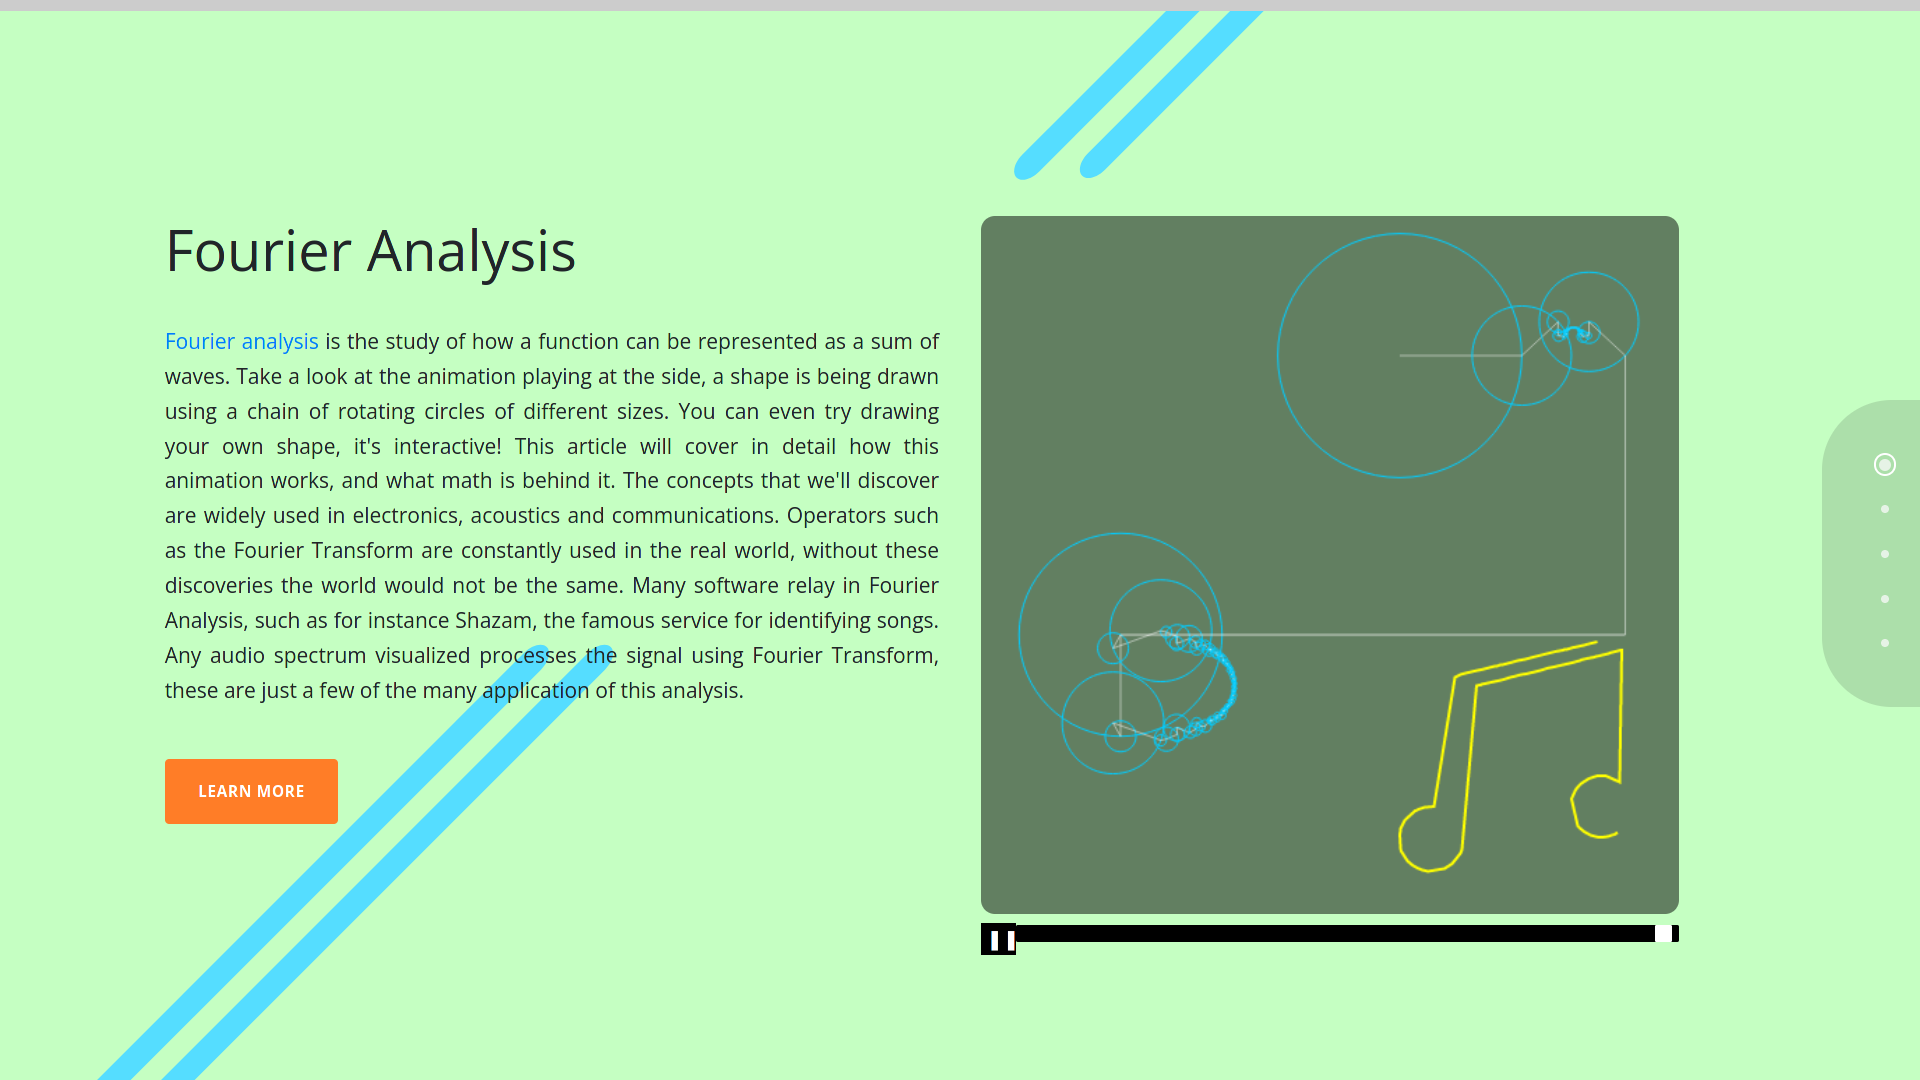
\includegraphics[width=\textwidth]{chap1.png}

\subsubsection{Requirements}

What are the requirements to read the article.

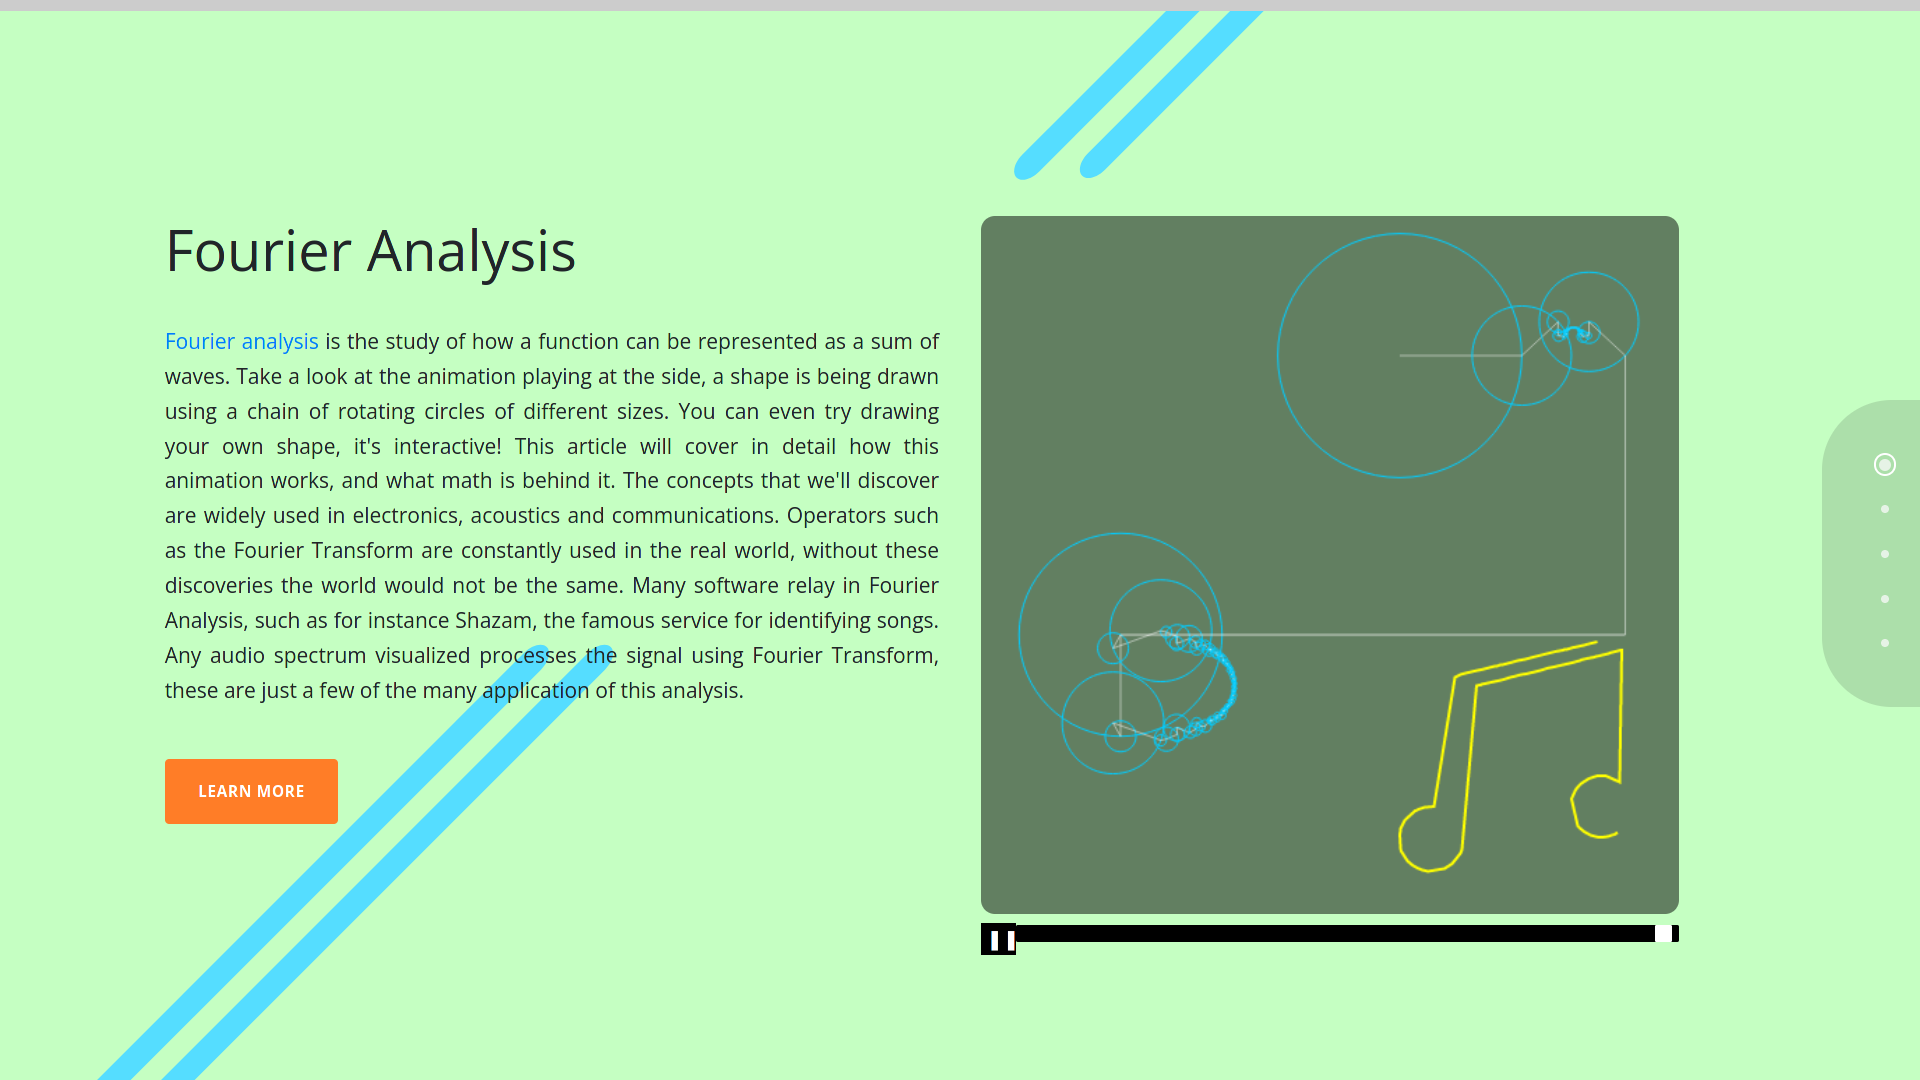
\includegraphics[width=\textwidth]{chap1.png}

\subsubsection{Introduction}

Who was Joseph Fourier and what he had discovered.

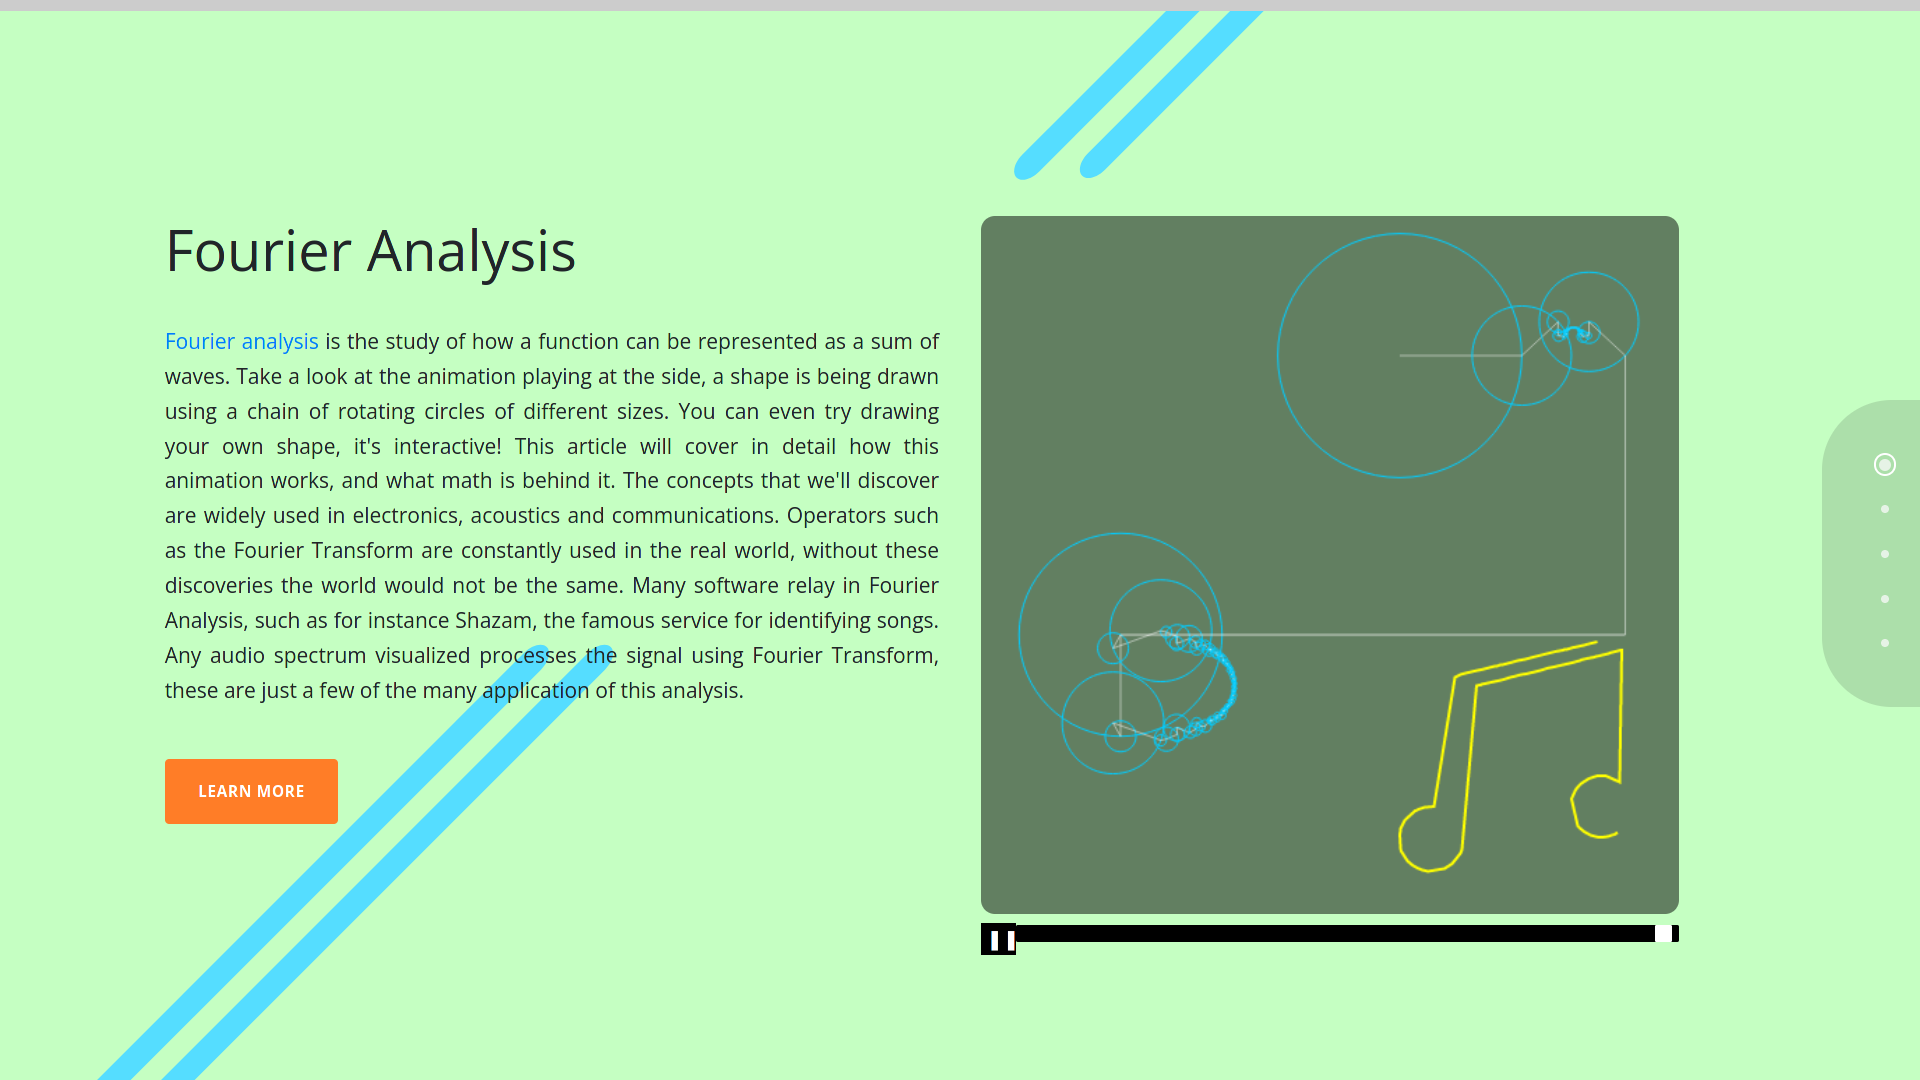
\includegraphics[width=\textwidth]{chap1.png}

\subsubsection{Fourier Series vs Fourier Transform}

What is the difference between the Furier series and the Fourier transform.

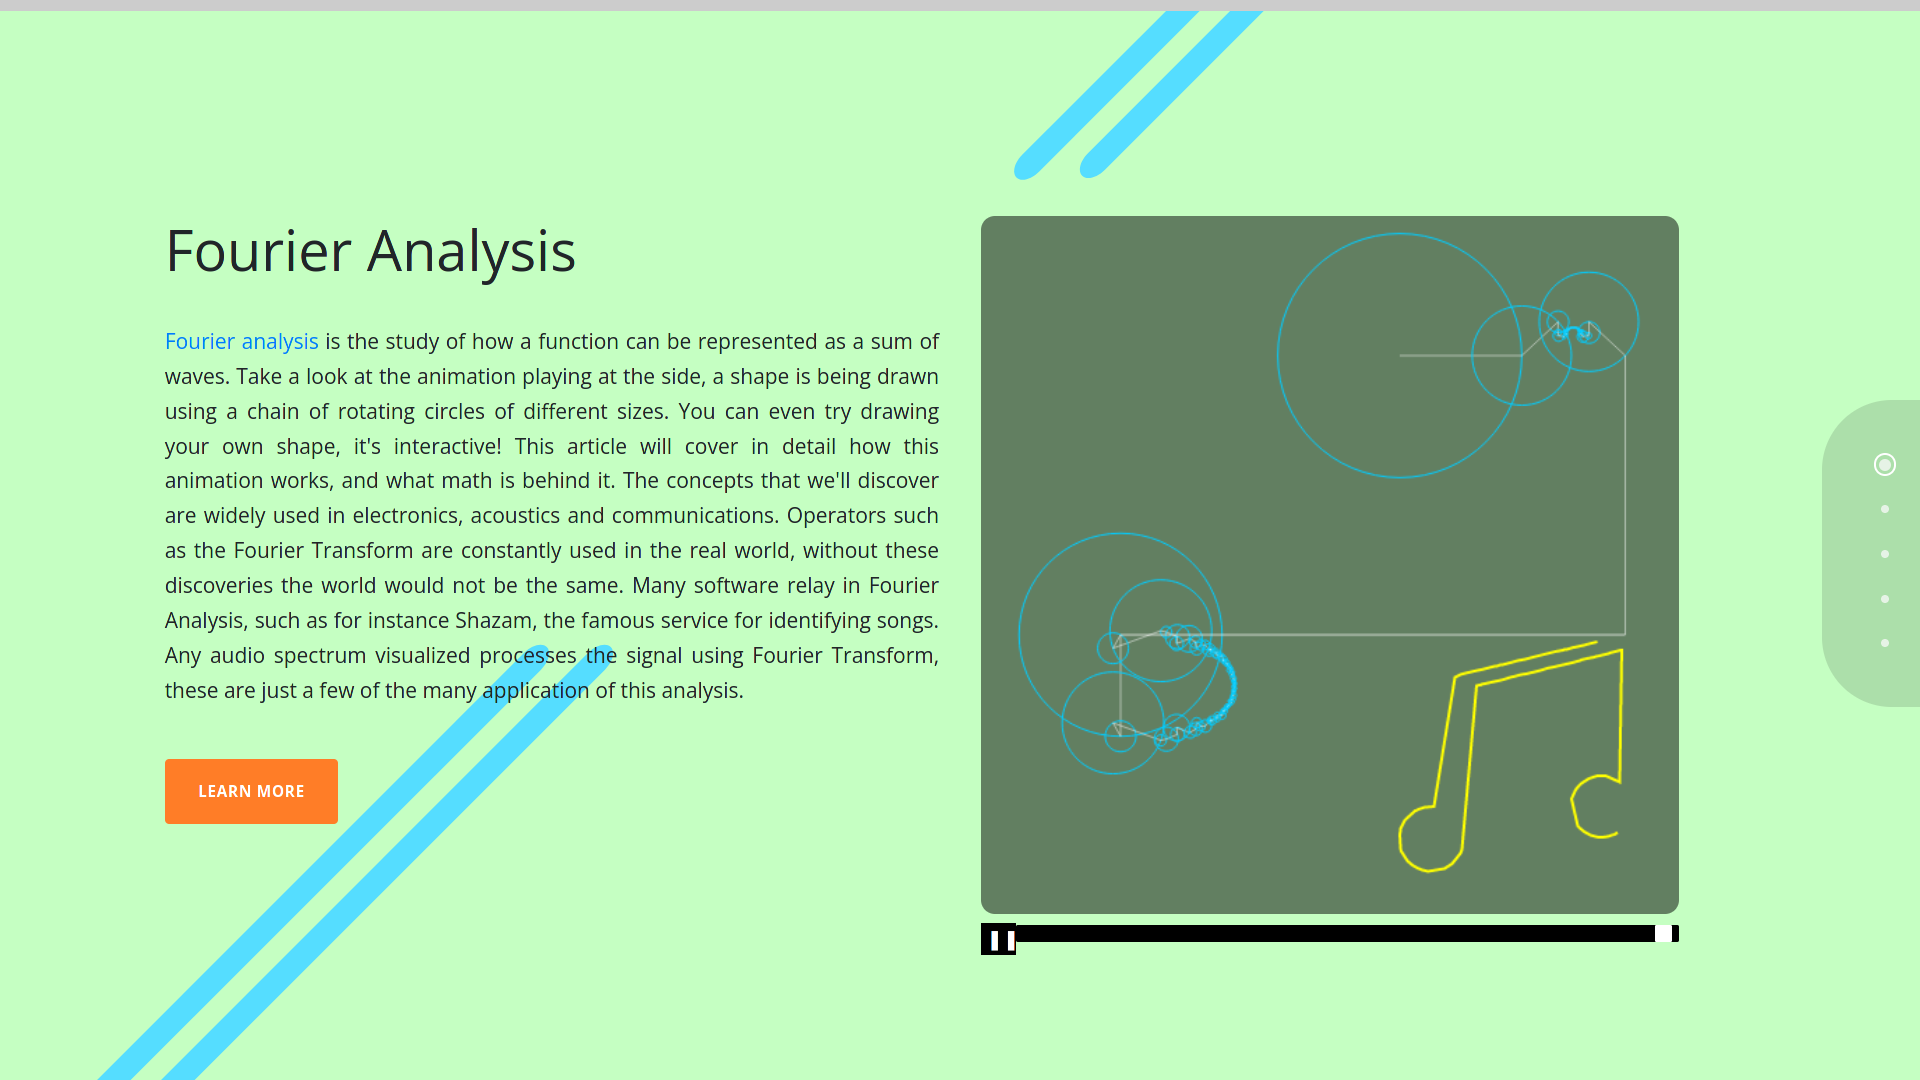
\includegraphics[width=\textwidth]{chap1.png}

\subsubsection{Trigonometric Fourier Series}

Representing a periodic function using a sum of trigonometric functions.

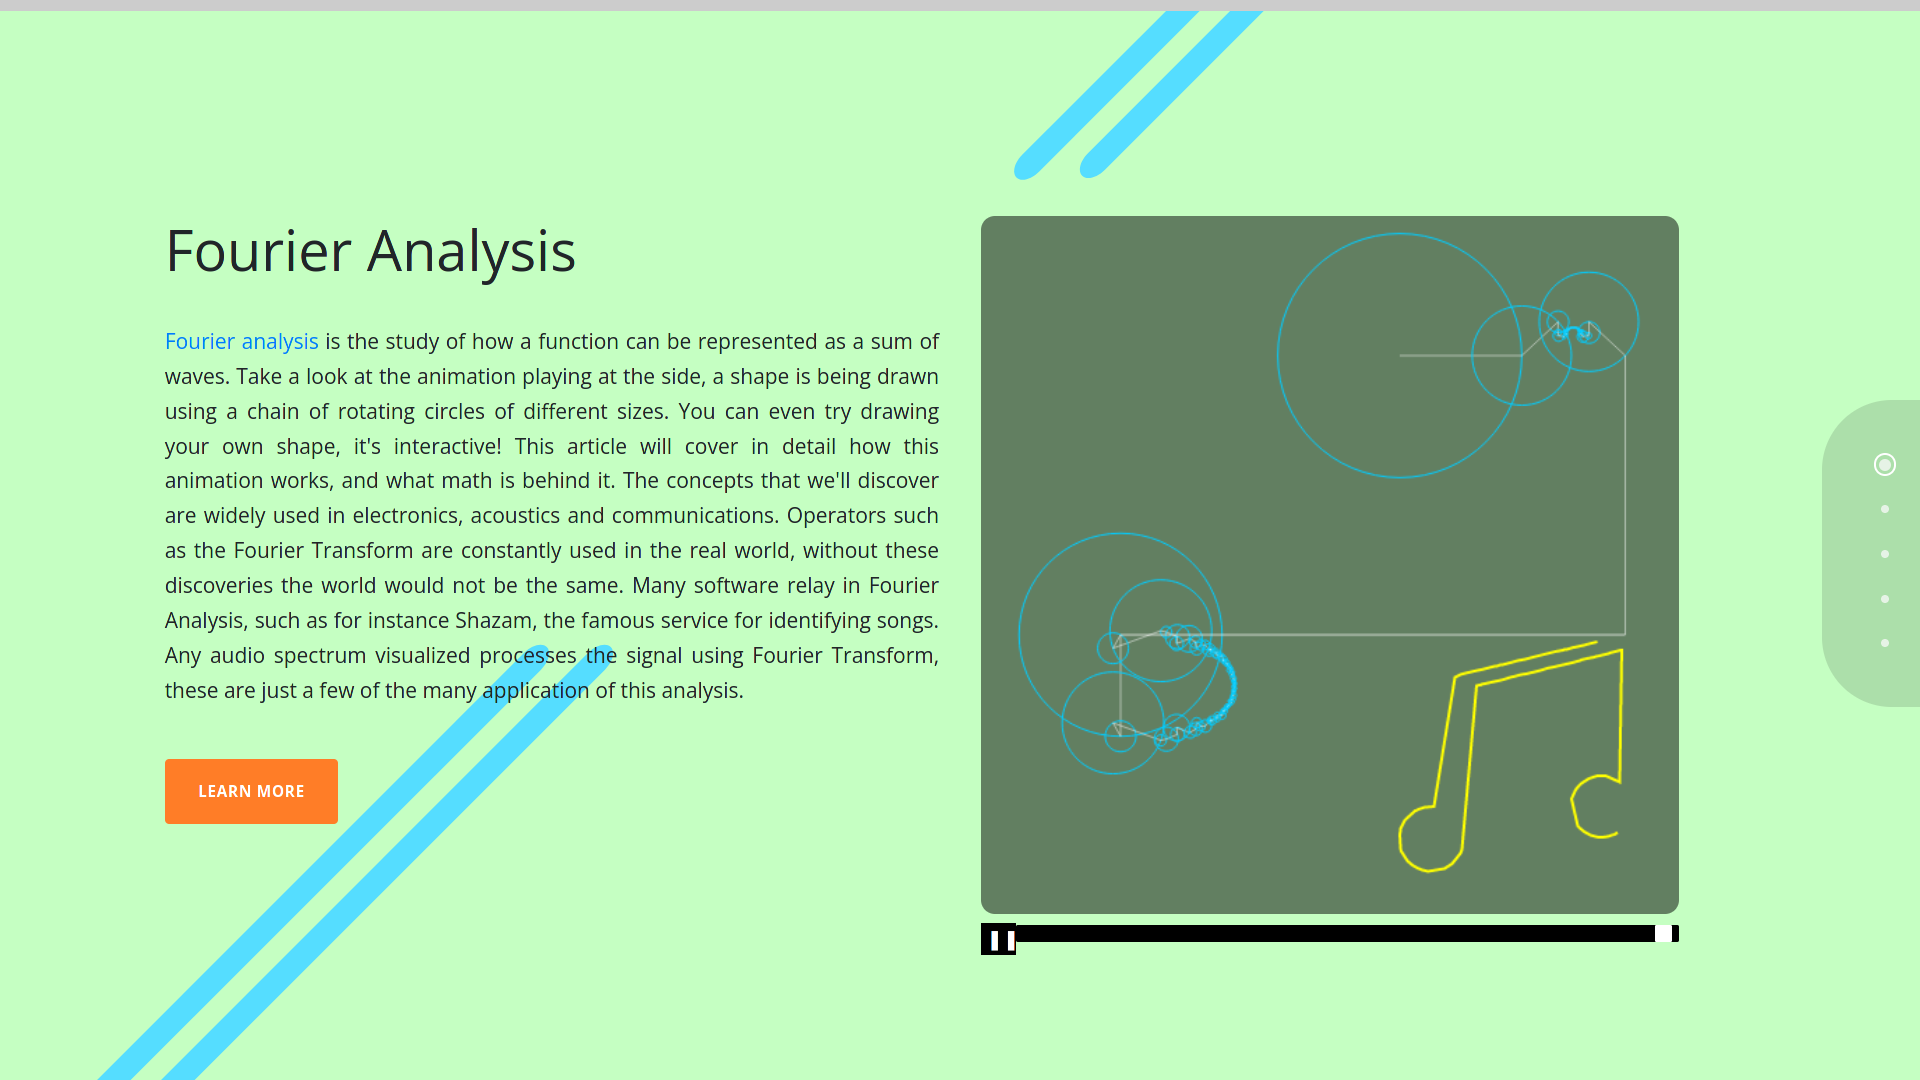
\includegraphics[width=\textwidth]{chap1.png}

\subsubsection{Trigonometric Fourier Series - C term}

Finding the \(C\) term.

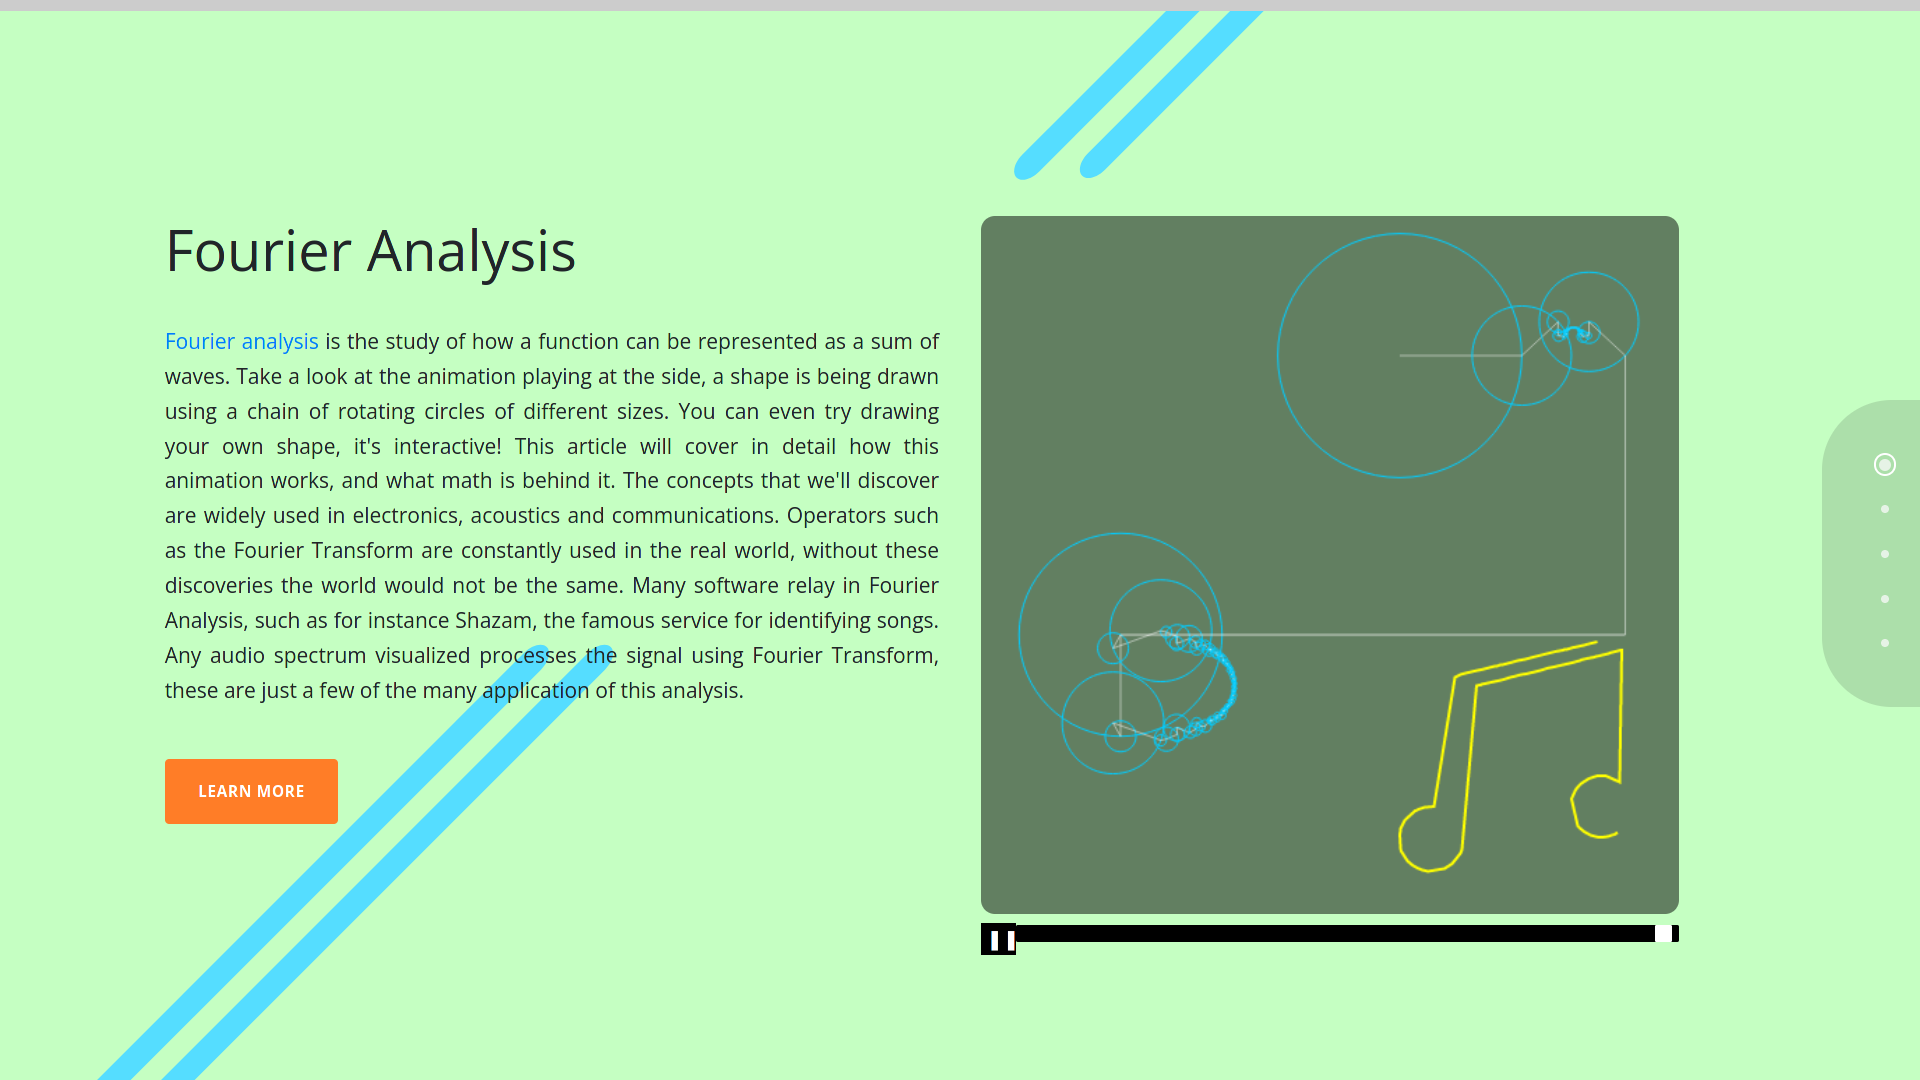
\includegraphics[width=\textwidth]{chap1.png}

\subsubsection{Trigonometric Fourier Series - Coefficients}

Finding the coefficients \(a_n\) and \(b_n\).

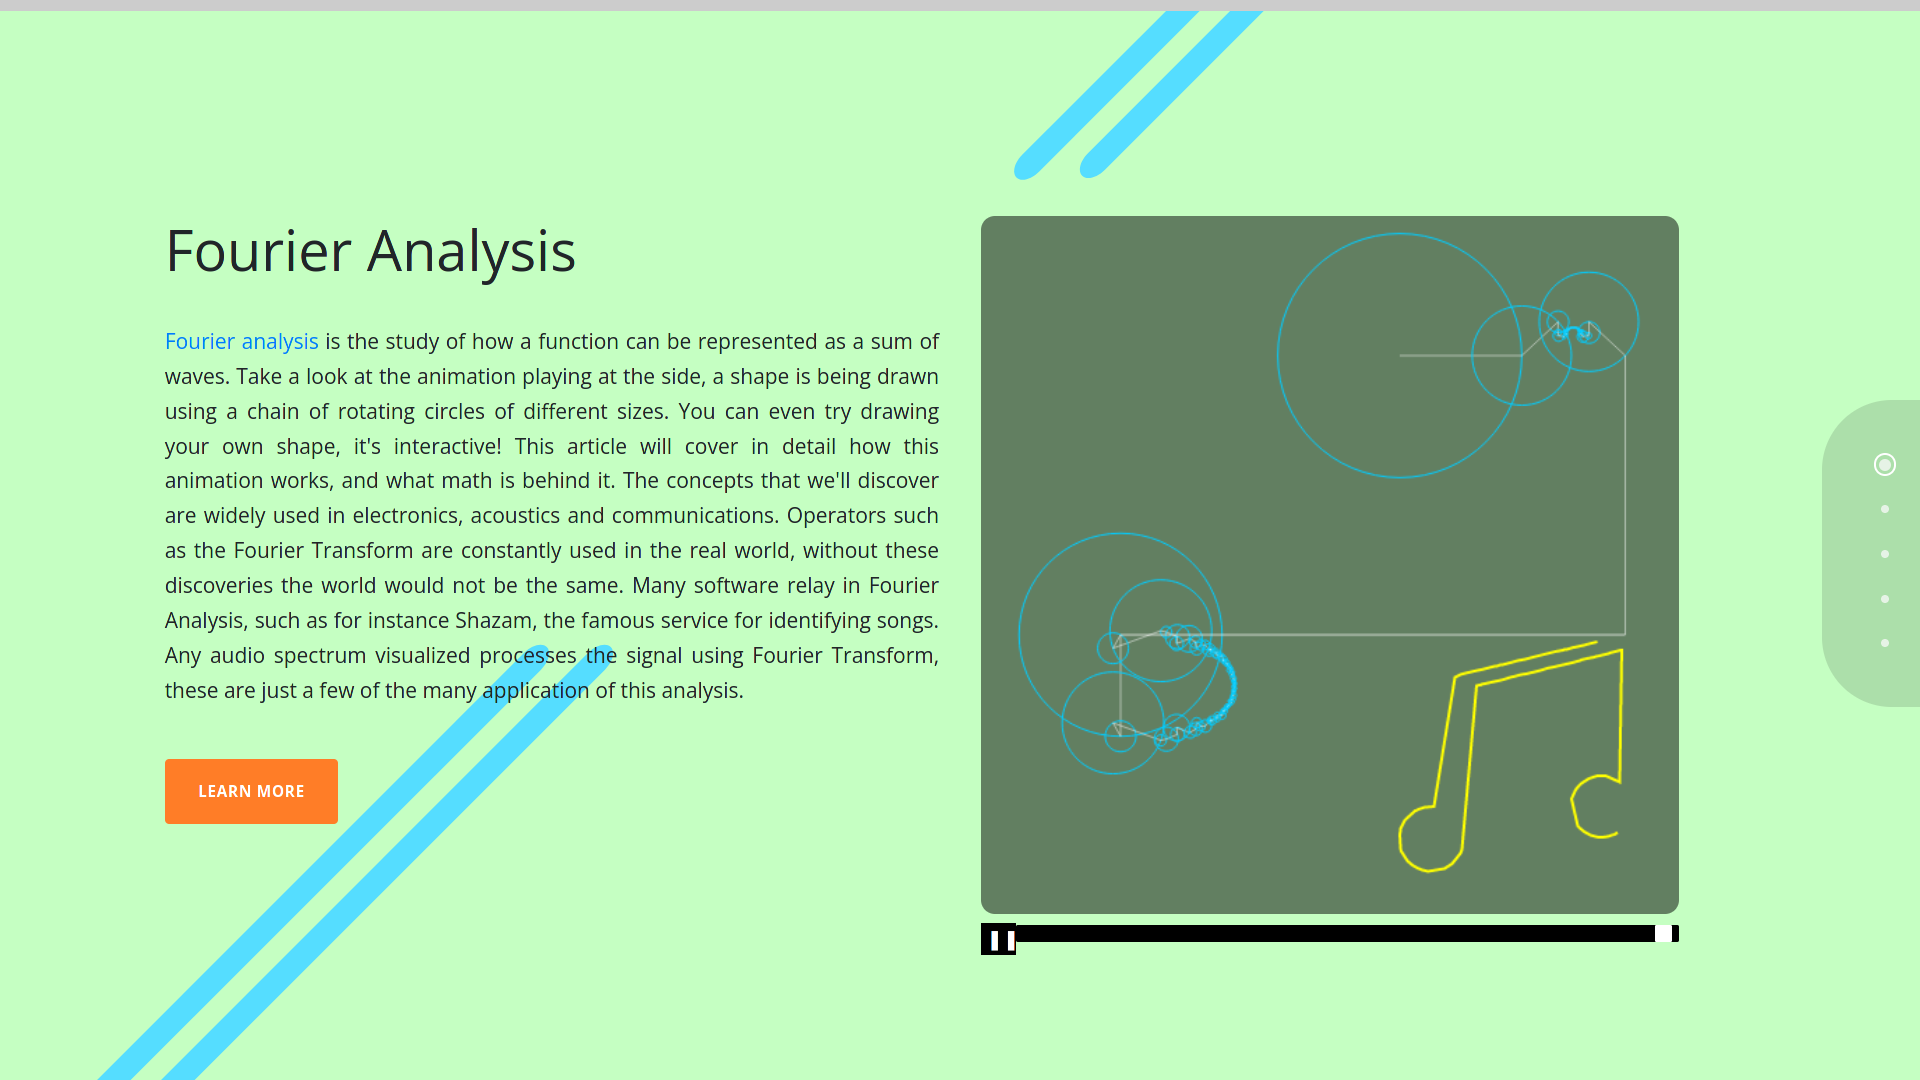
\includegraphics[width=\textwidth]{chap1.png}

\subsubsection{Fourier Series - Conclusion}

Conclusion on the last chapters.

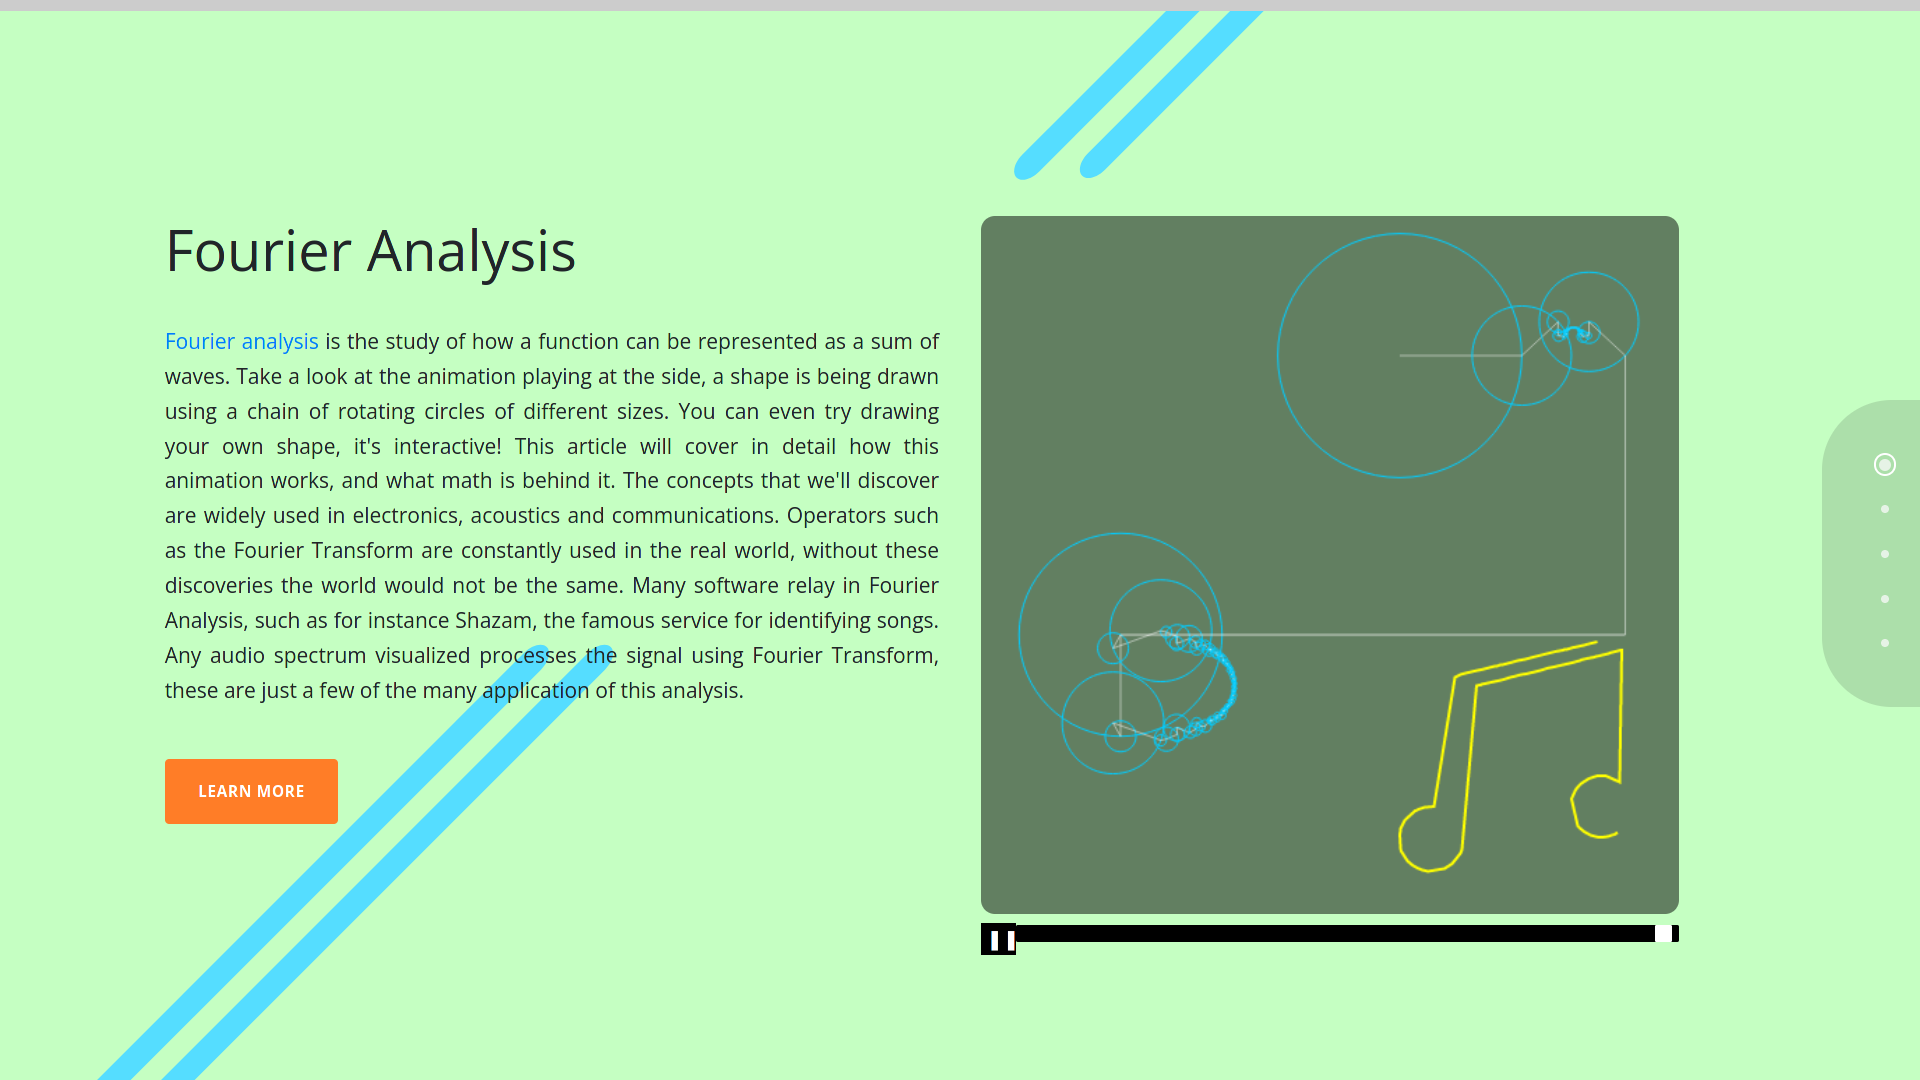
\includegraphics[width=\textwidth]{chap1.png}

\subsubsection{Main ideas - Complex plotting}

Plotting a function around the origin in the complex plane using Euler's identity.

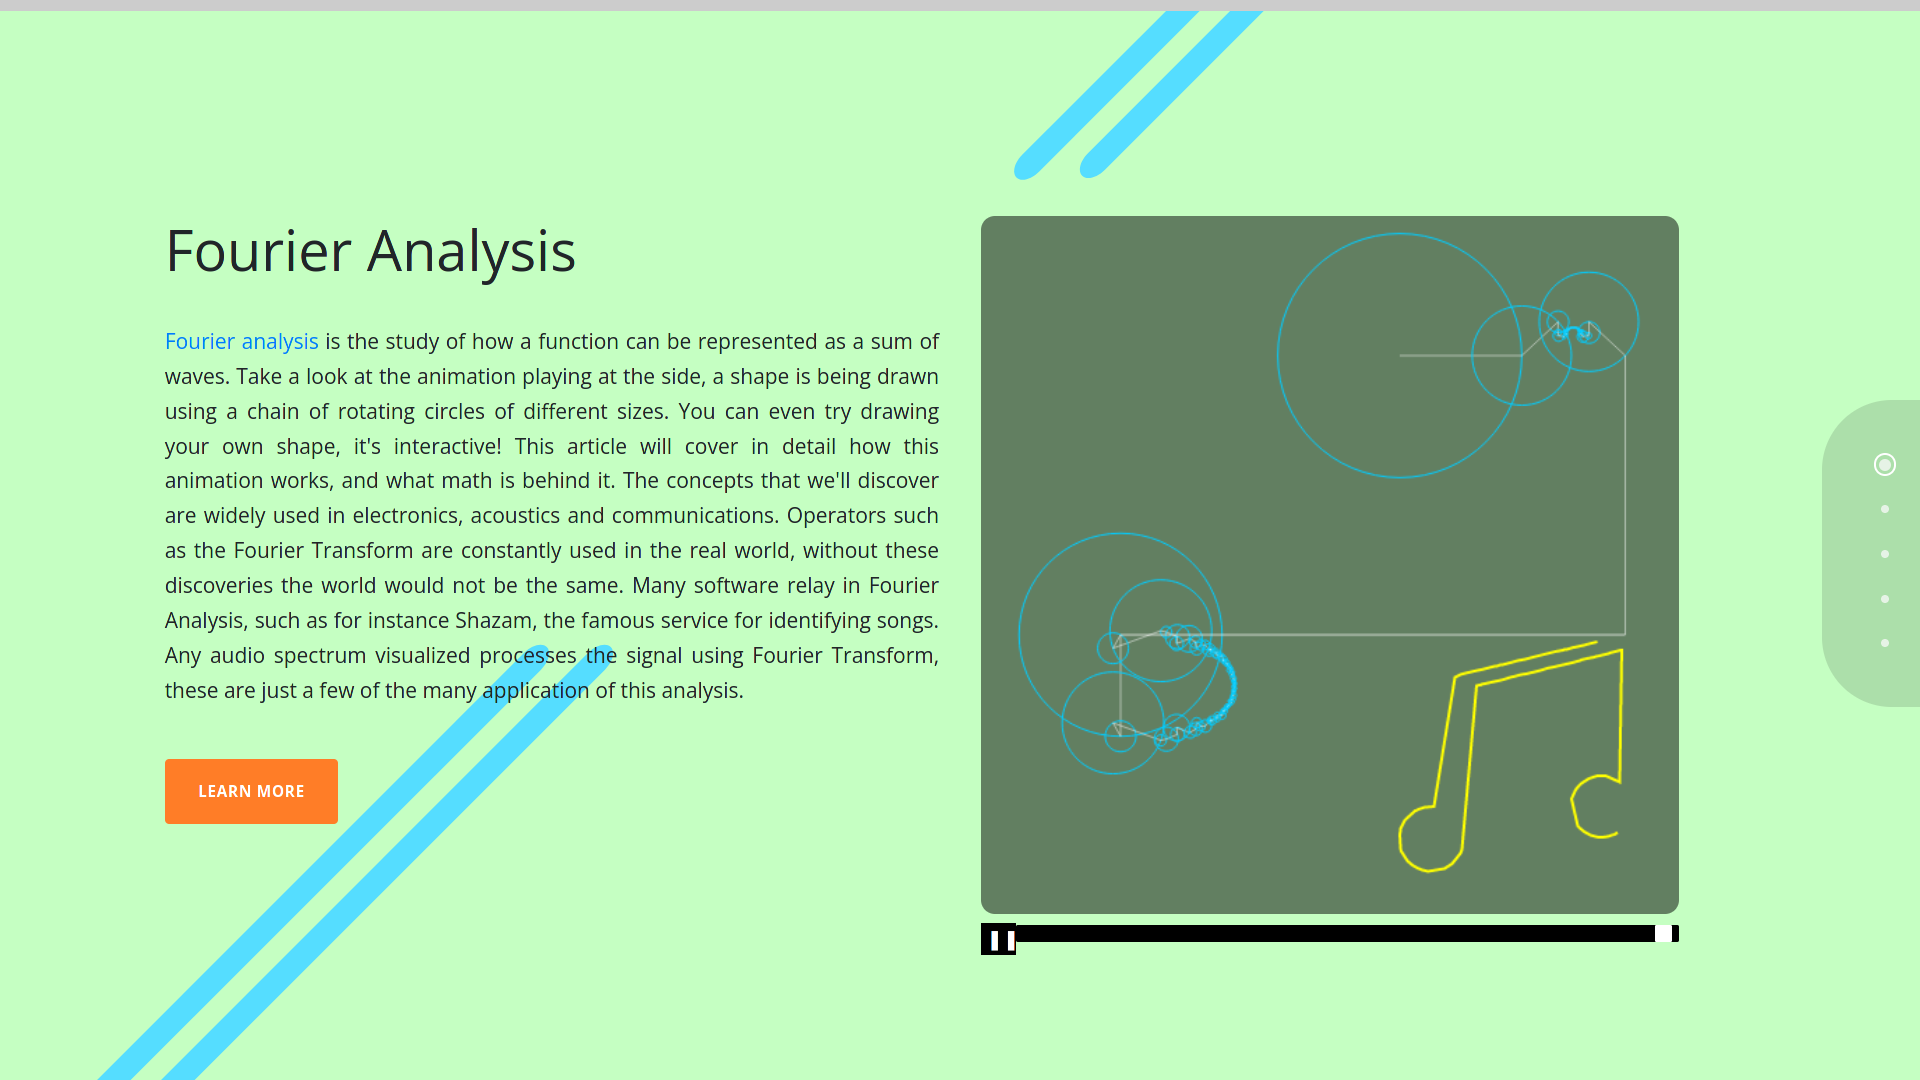
\includegraphics[width=\textwidth]{chap1.png}

\subsubsection{Main ideas - Center of mass}

Computing the center of mass of \(f(t)e^{-2\pi ti\xi}\)

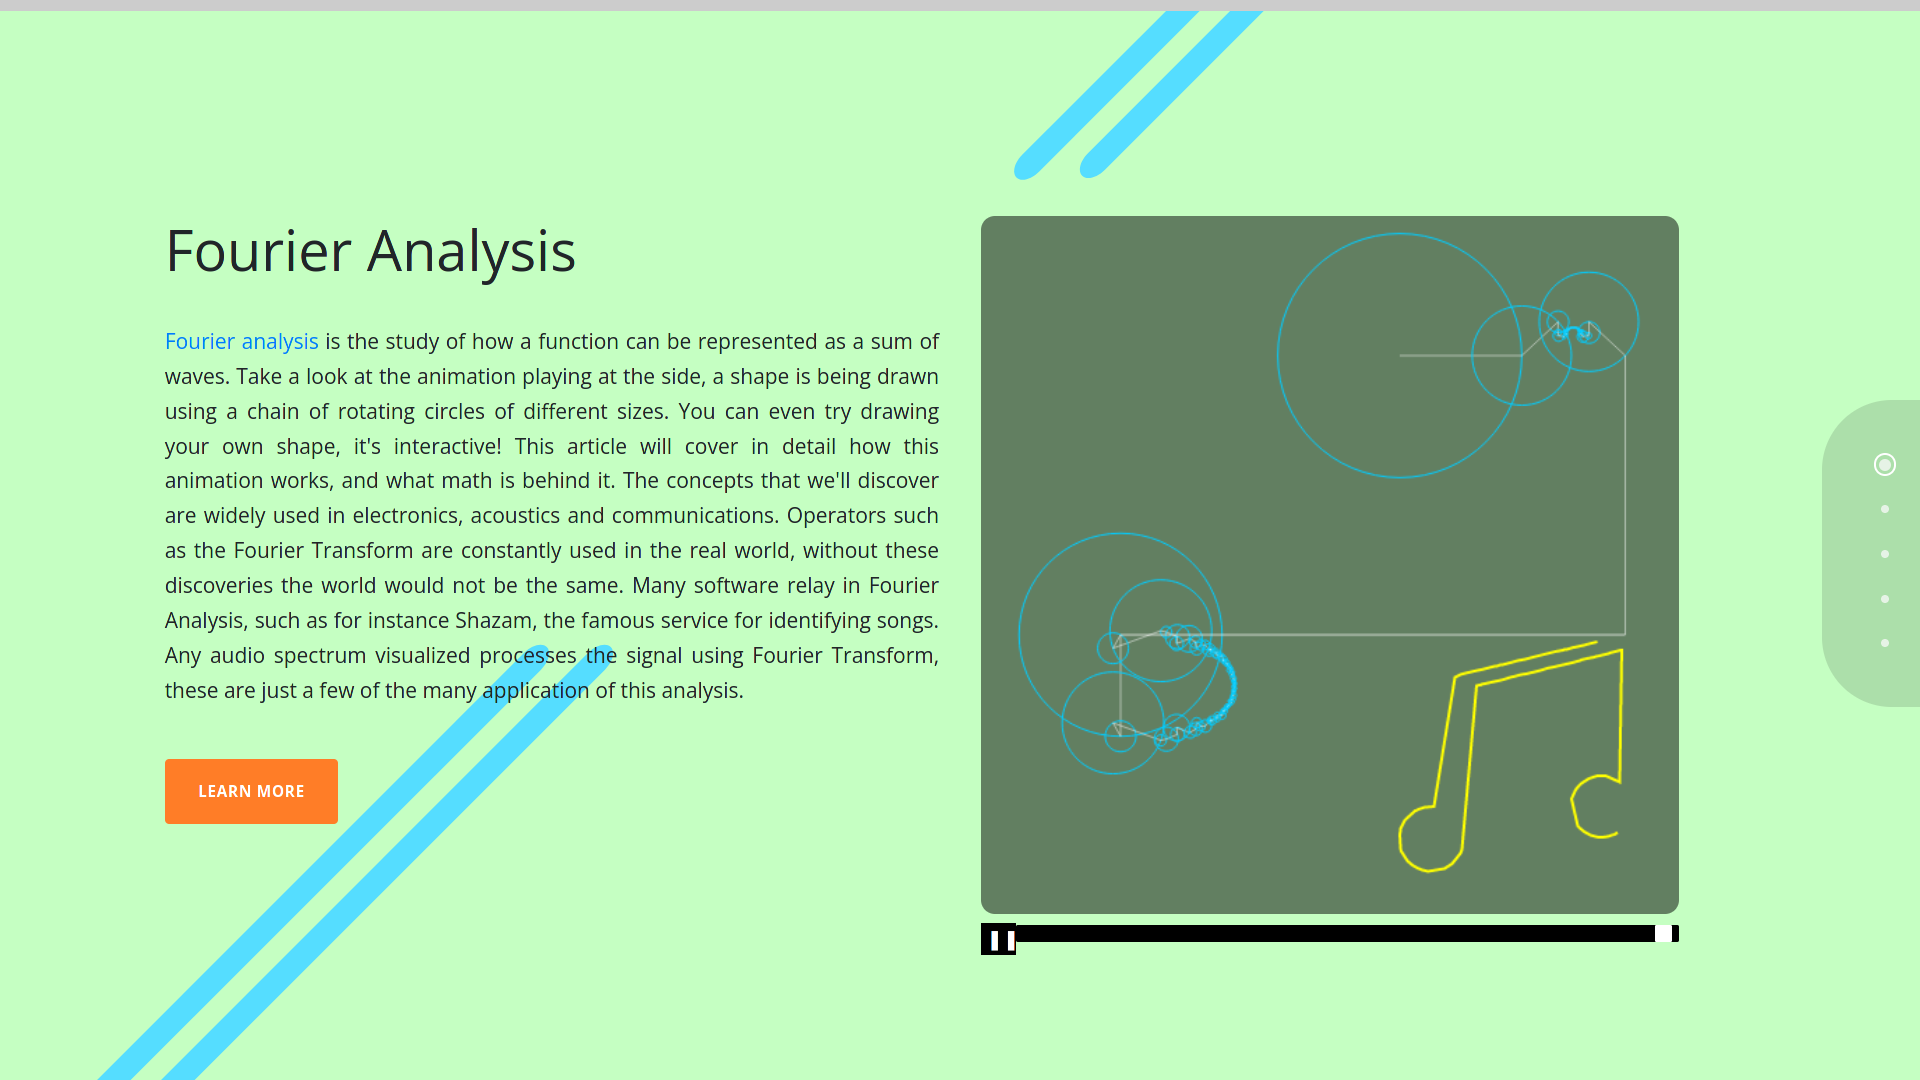
\includegraphics[width=\textwidth]{chap1.png}

\subsubsection{Main ideas - Fourier Transform}

What is the Fourier transform operator.

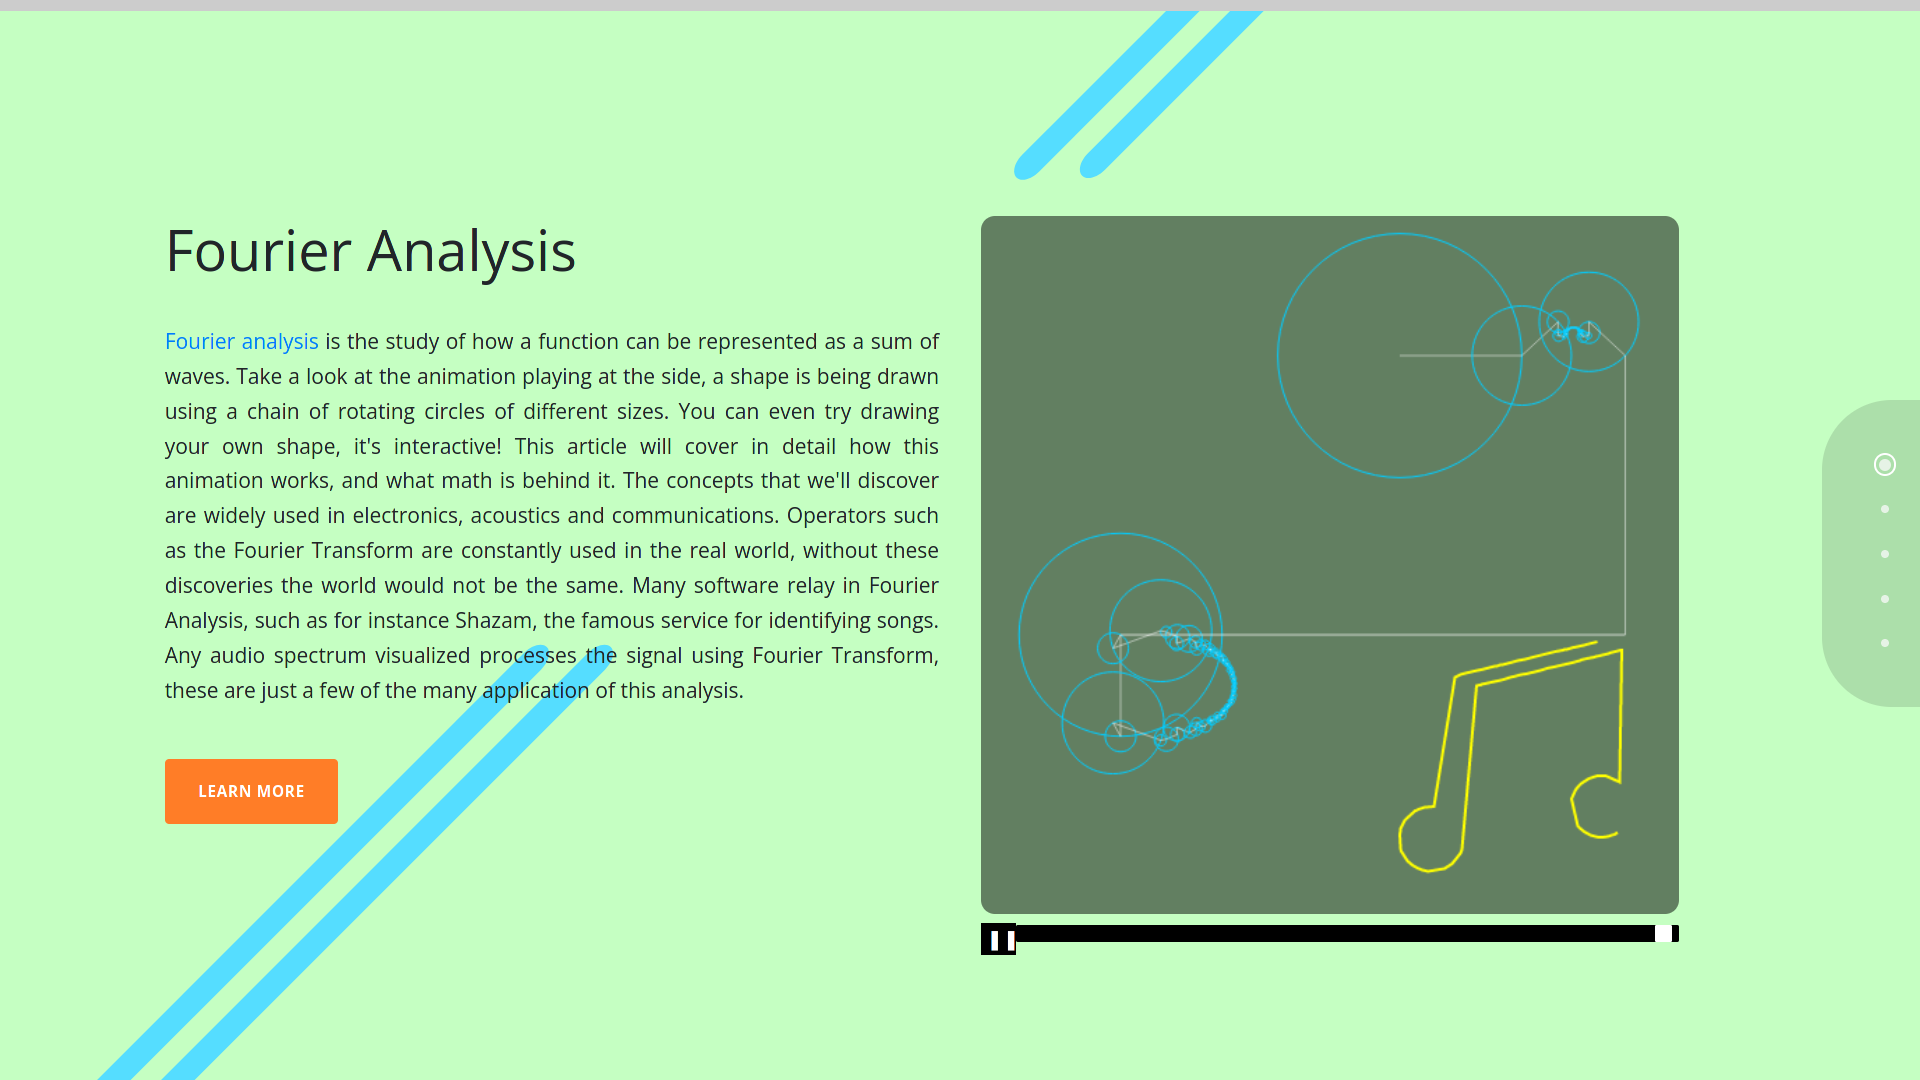
\includegraphics[width=\textwidth]{chap1.png}

\subsubsection{A Simple Example}

Computing the Fourier series of a simple function.

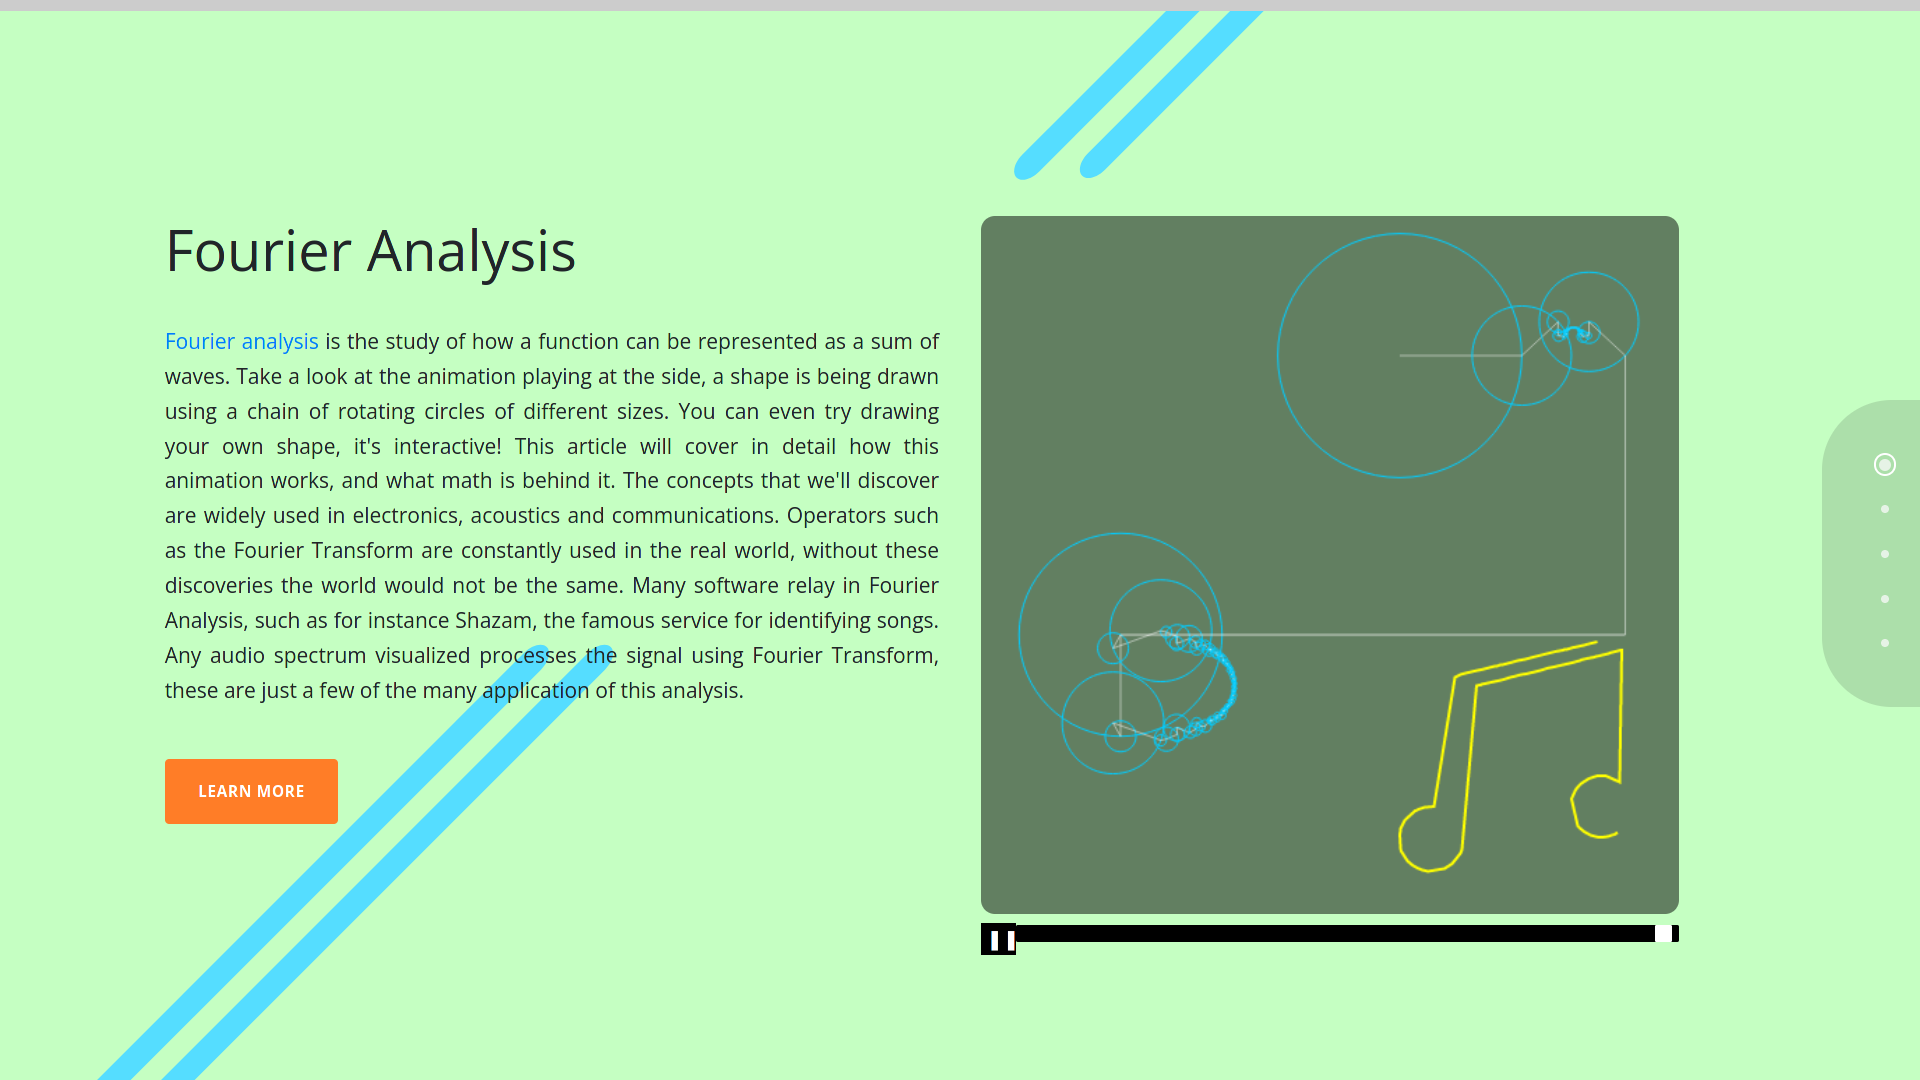
\includegraphics[width=\textwidth]{chap1.png}

\subsubsection{A Simple Example - Coefficients}

Finding the coefficients of the Fourier series.

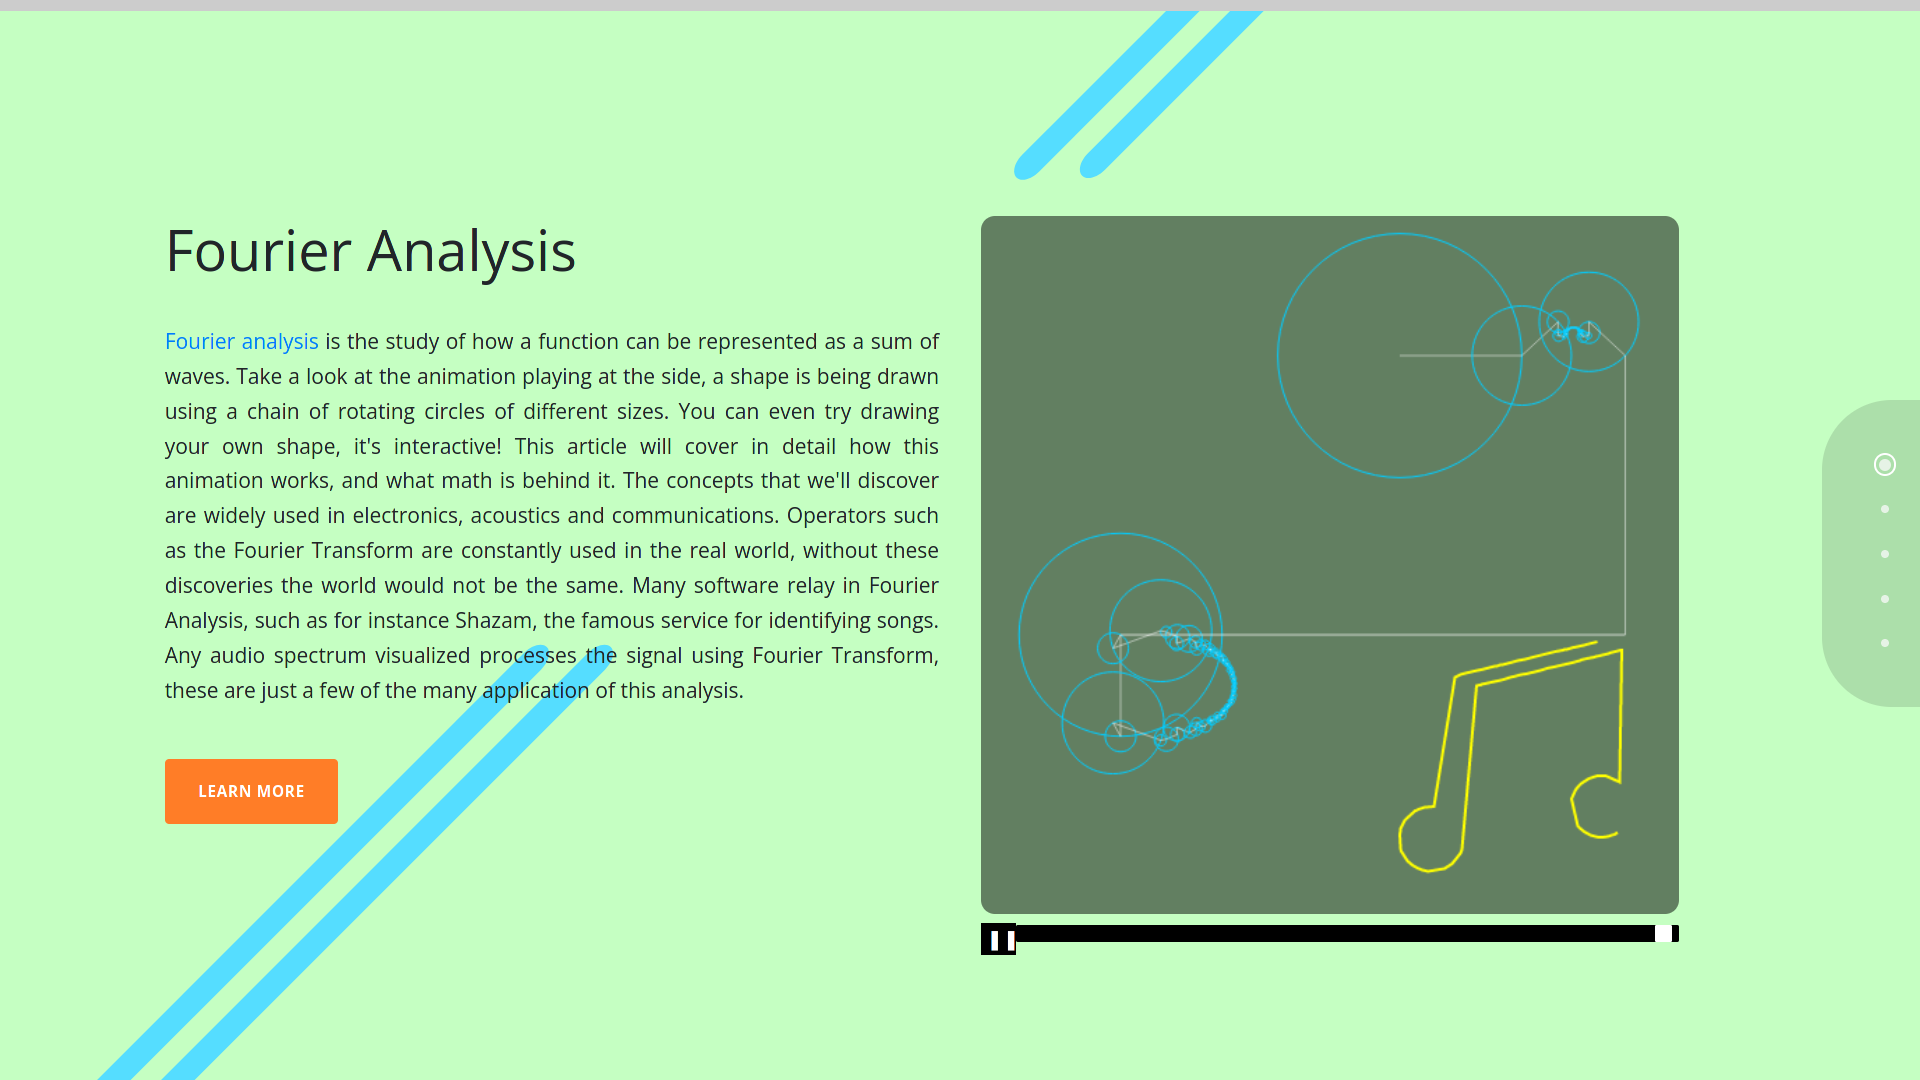
\includegraphics[width=\textwidth]{chap1.png}

\subsubsection{A Simple Example - Conclusion}

Demostrating the Fourier series by plotting it.

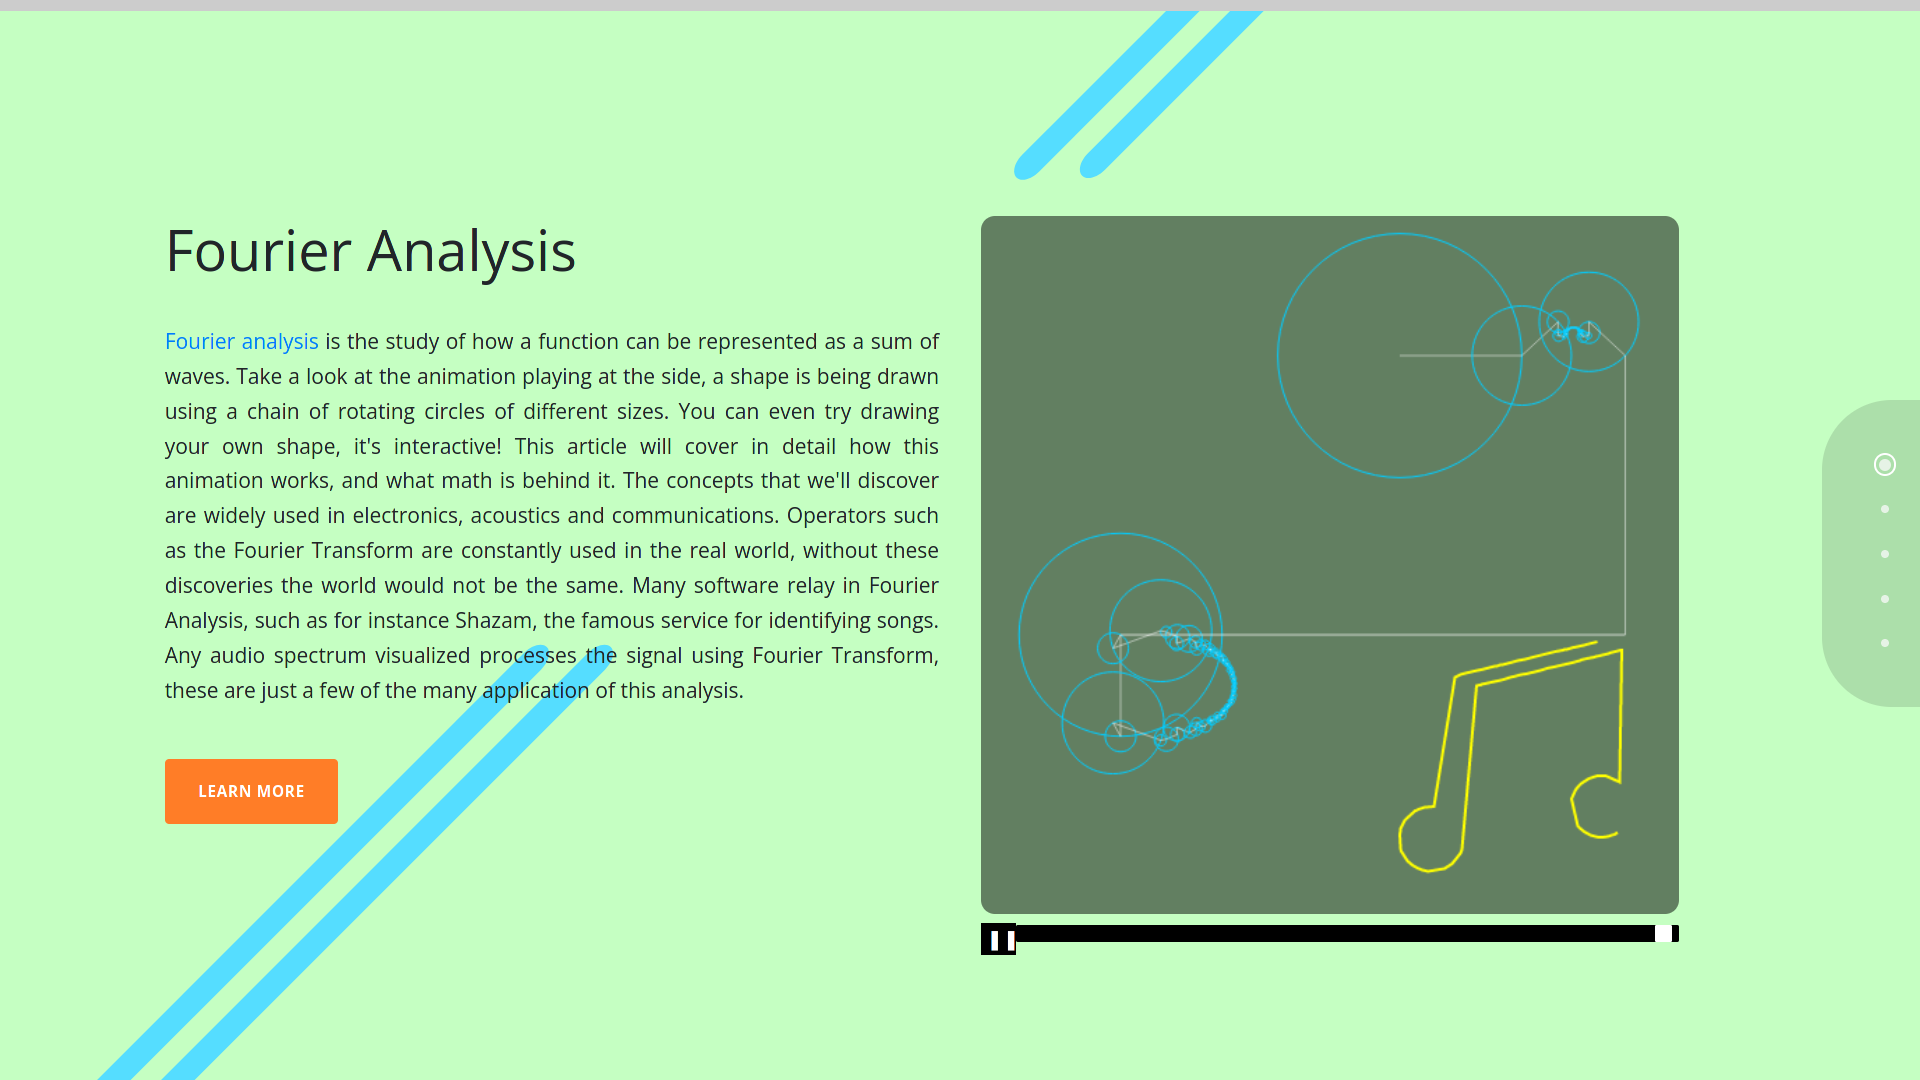
\includegraphics[width=\textwidth]{chap1.png}

\subsubsection{Exponential Fourier Series}

Defining the Fourier series using Euler's Identity.

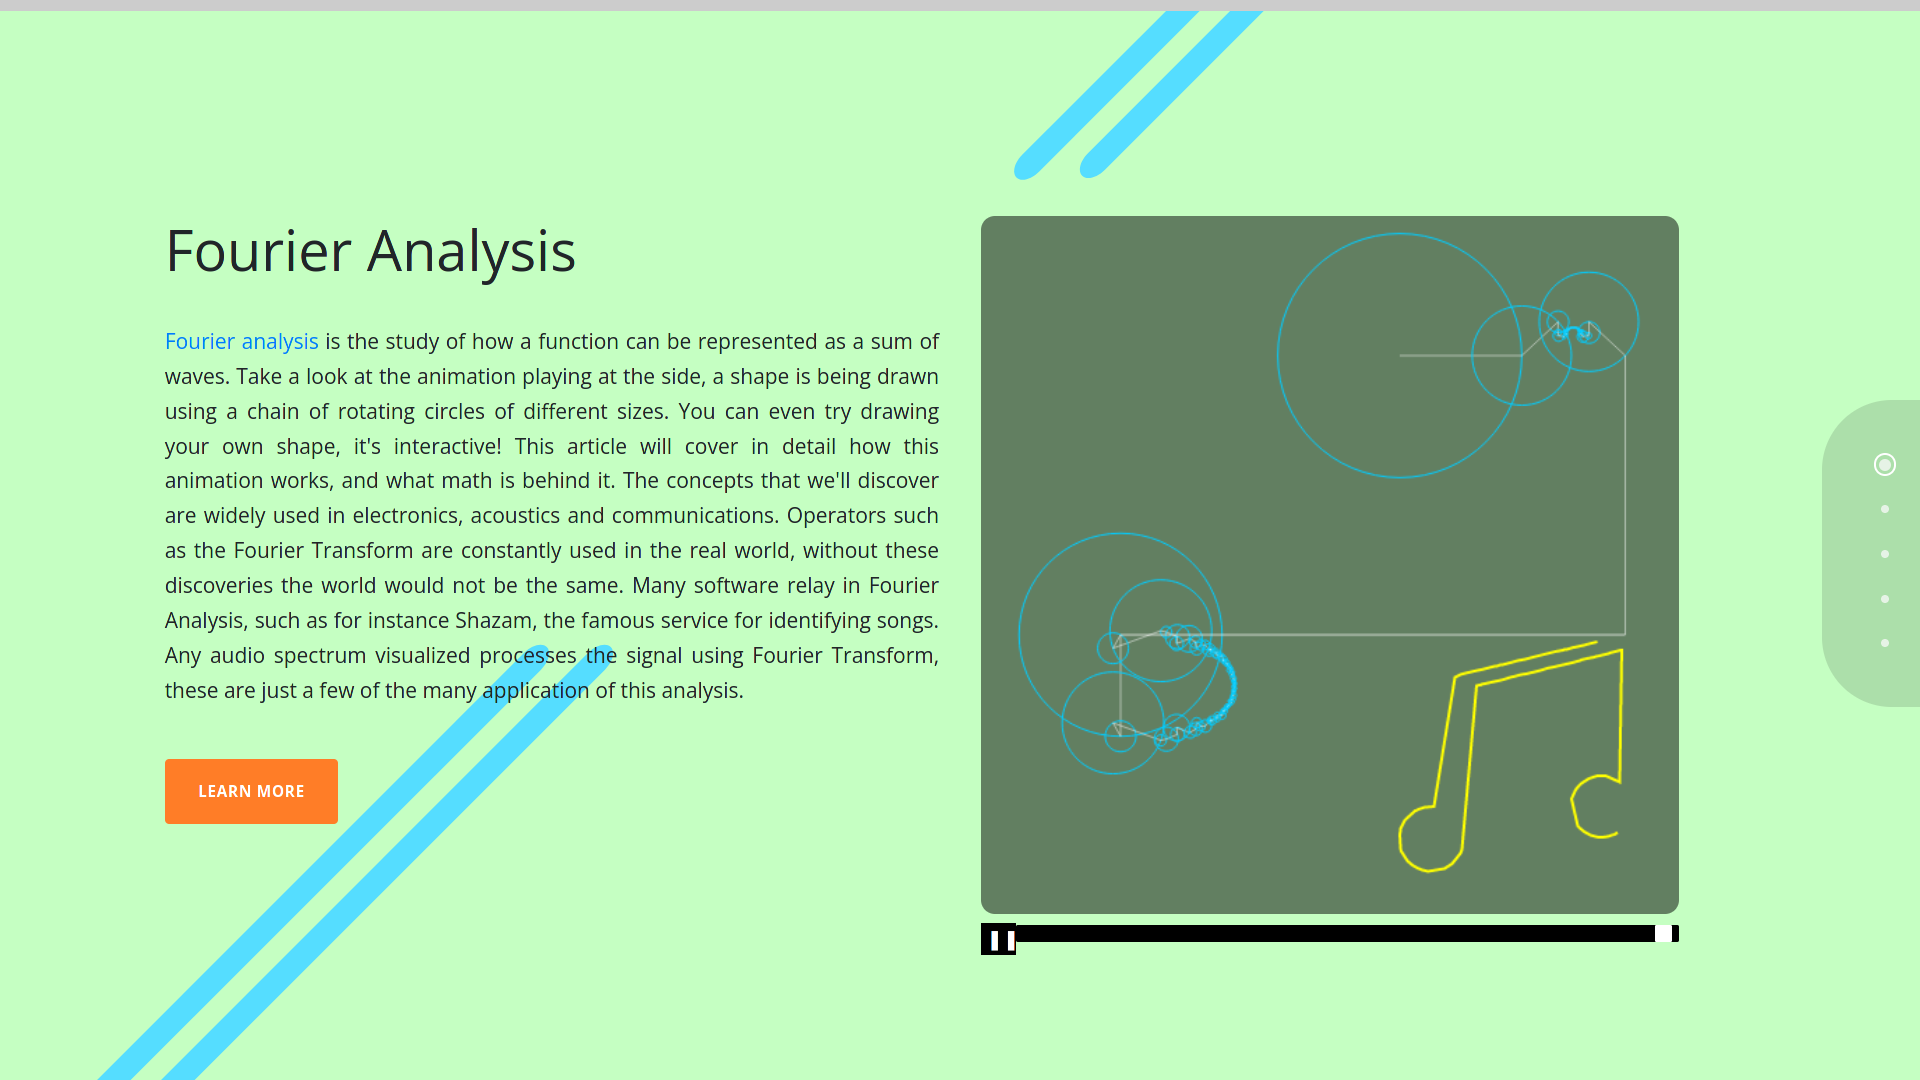
\includegraphics[width=\textwidth]{chap1.png}

\subsubsection{Fast Fourier Transform}

What is the Fast Fourier Transform algorithm.

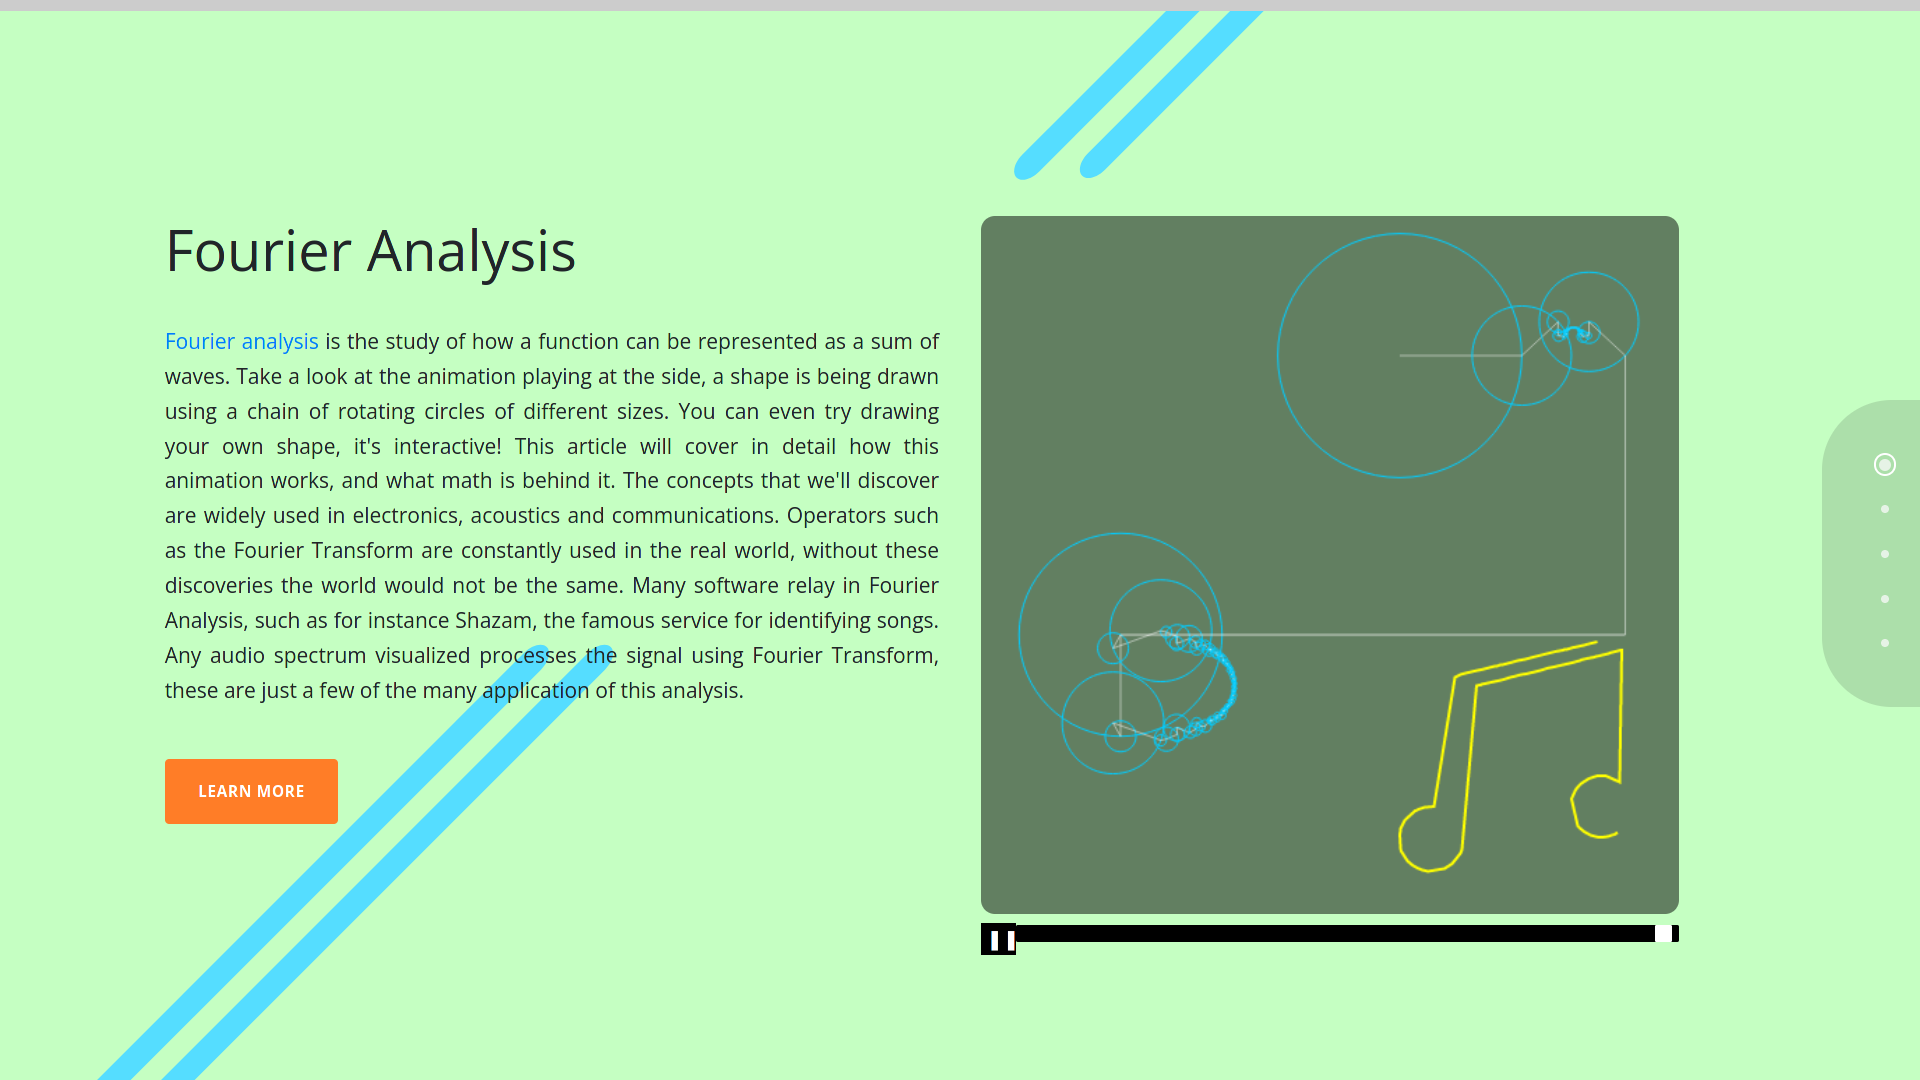
\includegraphics[width=\textwidth]{chap1.png}

\subsubsection{Conclusion}

How the animation in Chapter. 1 works.

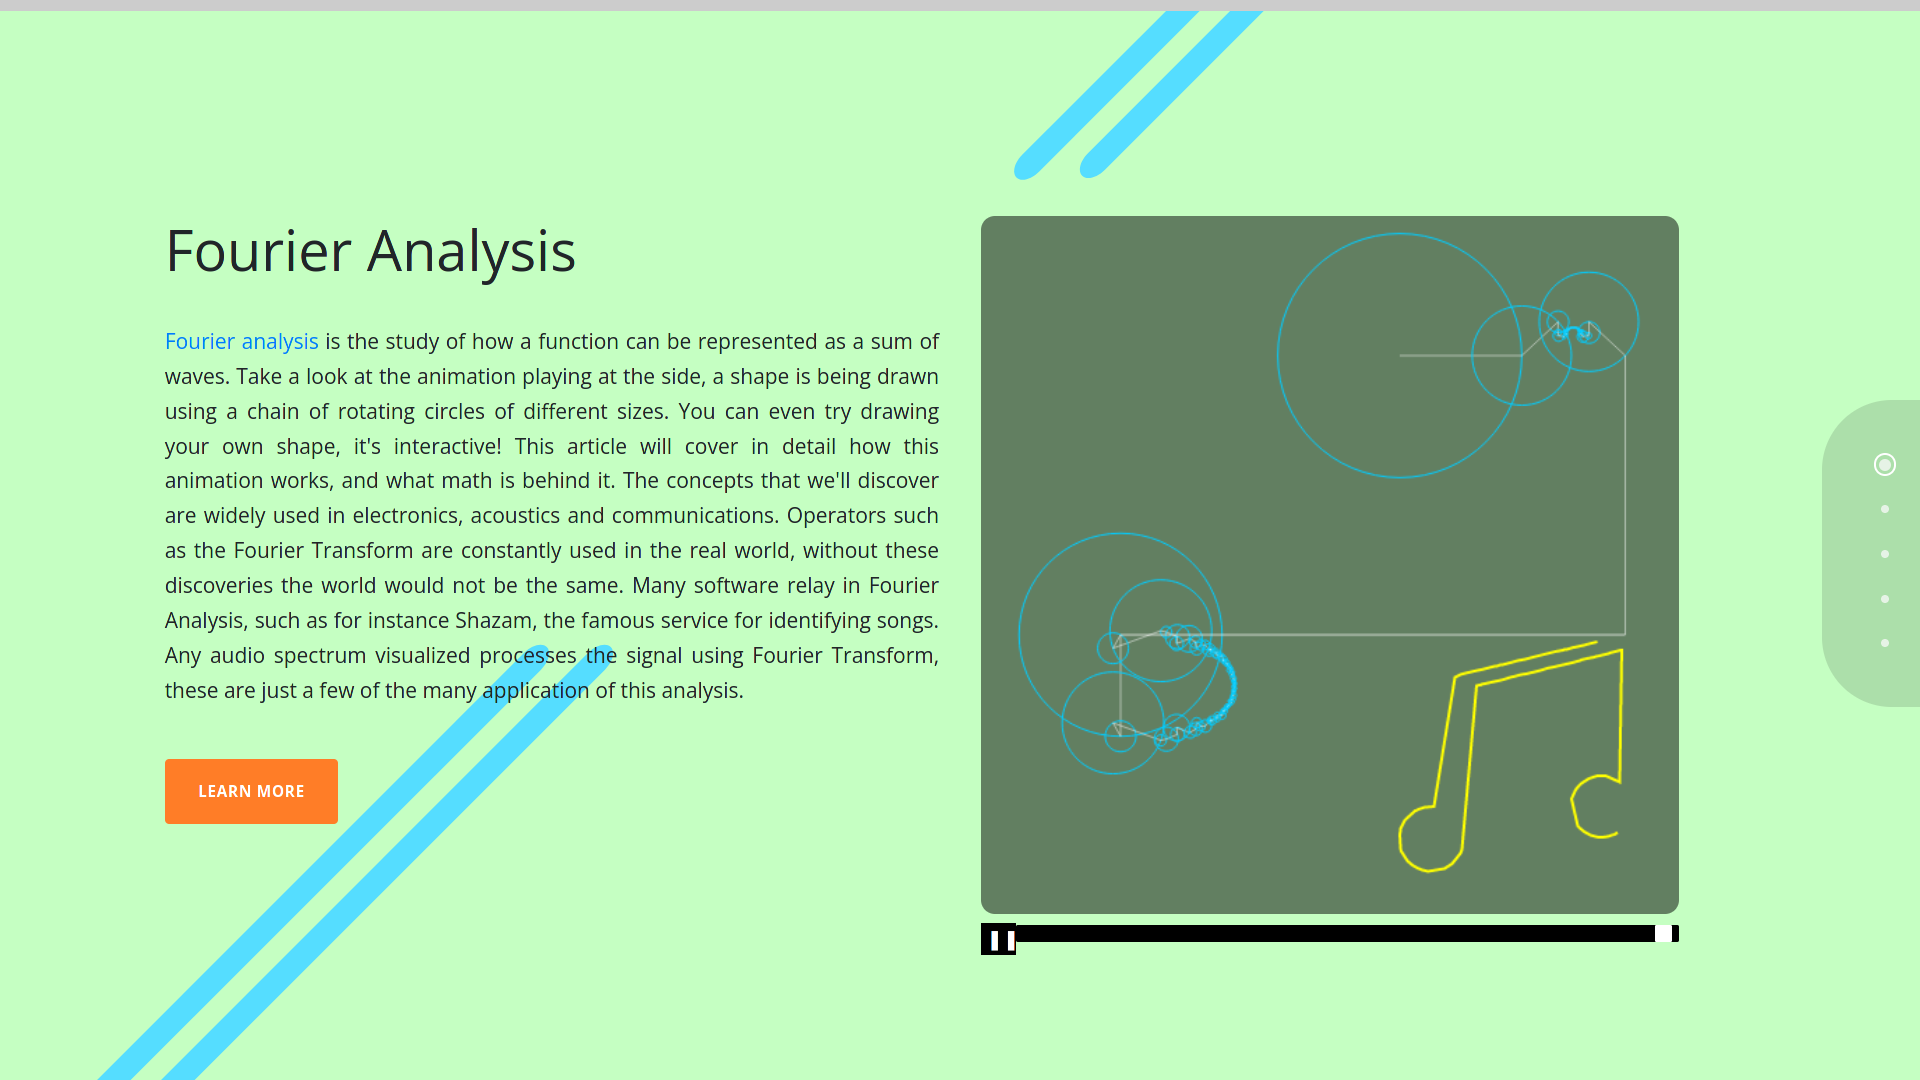
\includegraphics[width=\textwidth]{chap1.png}

\pagebreak

\subsection{Interactive Boxes Implementations}

\subsubsection{Fourier Series 1D}

\subsubsection{Fourier Series 2D}

\subsubsection{Complex Plot}

\subsubsection{Center of mass}

\subsubsection{Fourier Transform}

\end{document}